\documentclass[twoside]{book}

% Packages required by doxygen
\usepackage{fixltx2e}
\usepackage{calc}
\usepackage{doxygen}
\usepackage[export]{adjustbox} % also loads graphicx
\usepackage{graphicx}
\usepackage[utf8]{inputenc}
\usepackage{makeidx}
\usepackage{multicol}
\usepackage{multirow}
\PassOptionsToPackage{warn}{textcomp}
\usepackage{textcomp}
\usepackage[nointegrals]{wasysym}
\usepackage[table]{xcolor}

% Font selection
\usepackage[T1]{fontenc}
\usepackage[scaled=.90]{helvet}
\usepackage{courier}
\usepackage{amssymb}
\usepackage{sectsty}
\renewcommand{\familydefault}{\sfdefault}
\allsectionsfont{%
  \fontseries{bc}\selectfont%
  \color{darkgray}%
}
\renewcommand{\DoxyLabelFont}{%
  \fontseries{bc}\selectfont%
  \color{darkgray}%
}
\newcommand{\+}{\discretionary{\mbox{\scriptsize$\hookleftarrow$}}{}{}}

% Page & text layout
\usepackage{geometry}
\geometry{%
  a4paper,%
  top=2.5cm,%
  bottom=2.5cm,%
  left=2.5cm,%
  right=2.5cm%
}
\tolerance=750
\hfuzz=15pt
\hbadness=750
\setlength{\emergencystretch}{15pt}
\setlength{\parindent}{0cm}
\setlength{\parskip}{3ex plus 2ex minus 2ex}
\makeatletter
\renewcommand{\paragraph}{%
  \@startsection{paragraph}{4}{0ex}{-1.0ex}{1.0ex}{%
    \normalfont\normalsize\bfseries\SS@parafont%
  }%
}
\renewcommand{\subparagraph}{%
  \@startsection{subparagraph}{5}{0ex}{-1.0ex}{1.0ex}{%
    \normalfont\normalsize\bfseries\SS@subparafont%
  }%
}
\makeatother

% Headers & footers
\usepackage{fancyhdr}
\pagestyle{fancyplain}
\fancyhead[LE]{\fancyplain{}{\bfseries\thepage}}
\fancyhead[CE]{\fancyplain{}{}}
\fancyhead[RE]{\fancyplain{}{\bfseries\leftmark}}
\fancyhead[LO]{\fancyplain{}{\bfseries\rightmark}}
\fancyhead[CO]{\fancyplain{}{}}
\fancyhead[RO]{\fancyplain{}{\bfseries\thepage}}
\fancyfoot[LE]{\fancyplain{}{}}
\fancyfoot[CE]{\fancyplain{}{}}
\fancyfoot[RE]{\fancyplain{}{\bfseries\scriptsize Generated by Doxygen }}
\fancyfoot[LO]{\fancyplain{}{\bfseries\scriptsize Generated by Doxygen }}
\fancyfoot[CO]{\fancyplain{}{}}
\fancyfoot[RO]{\fancyplain{}{}}
\renewcommand{\footrulewidth}{0.4pt}
\renewcommand{\chaptermark}[1]{%
  \markboth{#1}{}%
}
\renewcommand{\sectionmark}[1]{%
  \markright{\thesection\ #1}%
}

% Indices & bibliography
\usepackage{natbib}
\usepackage[titles]{tocloft}
\setcounter{tocdepth}{3}
\setcounter{secnumdepth}{5}
\makeindex

% Hyperlinks (required, but should be loaded last)
\usepackage{ifpdf}
\ifpdf
  \usepackage[pdftex,pagebackref=true]{hyperref}
\else
  \usepackage[ps2pdf,pagebackref=true]{hyperref}
\fi
\hypersetup{%
  colorlinks=true,%
  linkcolor=blue,%
  citecolor=blue,%
  unicode%
}

% Custom commands
\newcommand{\clearemptydoublepage}{%
  \newpage{\pagestyle{empty}\cleardoublepage}%
}

\usepackage{caption}
\captionsetup{labelsep=space,justification=centering,font={bf},singlelinecheck=off,skip=4pt,position=top}

%===== C O N T E N T S =====

\begin{document}

% Titlepage & ToC
\hypersetup{pageanchor=false,
             bookmarksnumbered=true,
             pdfencoding=unicode
            }
\pagenumbering{alph}
\begin{titlepage}
\vspace*{7cm}
\begin{center}%
{\Large Ti project laser turtle \\[1ex]\large V1.\+0 }\\
\vspace*{1cm}
{\large Generated by Doxygen 1.8.12}\\
\end{center}
\end{titlepage}
\clearemptydoublepage
\pagenumbering{roman}
\tableofcontents
\clearemptydoublepage
\pagenumbering{arabic}
\hypersetup{pageanchor=true}

%--- Begin generated contents ---
\chapter{Hierarchical Index}
\section{Class Hierarchy}
This inheritance list is sorted roughly, but not completely, alphabetically\+:\begin{DoxyCompactList}
\item \contentsline{section}{button}{\pageref{classbutton}}{}
\item \contentsline{section}{game\+\_\+information\+\_\+data}{\pageref{classgame__information__data}}{}
\item \contentsline{section}{hit}{\pageref{classhit}}{}
\item \contentsline{section}{ir\+\_\+message\+\_\+logic}{\pageref{classir__message__logic}}{}
\item \contentsline{section}{ir\+\_\+sender}{\pageref{classir__sender}}{}
\item \contentsline{section}{Keypad}{\pageref{class_keypad}}{}
\item \contentsline{section}{lcd\+\_\+display}{\pageref{classlcd__display}}{}
\item \contentsline{section}{lcd\+\_\+passthrough}{\pageref{structlcd__passthrough}}{}
\item \contentsline{section}{led\+\_\+color\+\_\+behaviour}{\pageref{structled__color__behaviour}}{}
\item \contentsline{section}{listener}{\pageref{classlistener}}{}
\begin{DoxyCompactList}
\item \contentsline{section}{button\+\_\+controller}{\pageref{classbutton__controller}}{}
\end{DoxyCompactList}
\item \contentsline{section}{my\+\_\+player\+\_\+information}{\pageref{classmy__player__information}}{}
\item \contentsline{section}{register\+\_\+game\+\_\+parameters\+\_\+controller}{\pageref{classregister__game__parameters__controller}}{}
\item \contentsline{section}{rgb\+\_\+led}{\pageref{classrgb__led}}{}
\item \contentsline{section}{sound\+\_\+lookup}{\pageref{structsound__lookup}}{}
\item \contentsline{section}{speaker}{\pageref{classspeaker}}{}
\item task\begin{DoxyCompactList}
\item \contentsline{section}{button\+\_\+controller}{\pageref{classbutton__controller}}{}
\item \contentsline{section}{game\+\_\+time\+\_\+controller}{\pageref{classgame__time__controller}}{}
\item \contentsline{section}{init\+\_\+game\+\_\+controller}{\pageref{classinit__game__controller}}{}
\item \contentsline{section}{ir\+\_\+receiver\+\_\+controller}{\pageref{classir__receiver__controller}}{}
\item \contentsline{section}{lcd\+\_\+display\+\_\+controller}{\pageref{classlcd__display__controller}}{}
\item \contentsline{section}{led\+\_\+controller}{\pageref{classled__controller}}{}
\item \contentsline{section}{run\+\_\+game\+\_\+controller}{\pageref{classrun__game__controller}}{}
\item \contentsline{section}{send\+\_\+controller}{\pageref{classsend__controller}}{}
\item \contentsline{section}{send\+\_\+controller}{\pageref{classsend__controller}}{}
\item \contentsline{section}{speaker\+\_\+controller}{\pageref{classspeaker__controller}}{}
\end{DoxyCompactList}
\end{DoxyCompactList}

\chapter{Class Index}
\section{Class List}
Here are the classes, structs, unions and interfaces with brief descriptions\+:\begin{DoxyCompactList}
\item\contentsline{section}{\hyperlink{classbutton}{button} \\*Button }{\pageref{classbutton}}{}
\item\contentsline{section}{\hyperlink{classbutton__controller}{button\+\_\+controller} \\*Button\+\_\+controller }{\pageref{classbutton__controller}}{}
\item\contentsline{section}{\hyperlink{classgame__information__data}{game\+\_\+information\+\_\+data} \\*Store game information }{\pageref{classgame__information__data}}{}
\item\contentsline{section}{\hyperlink{classgame__time__controller}{game\+\_\+time\+\_\+controller} \\*Game time controller }{\pageref{classgame__time__controller}}{}
\item\contentsline{section}{\hyperlink{classhit}{hit} \\*Store a hit }{\pageref{classhit}}{}
\item\contentsline{section}{\hyperlink{classinit__game__controller}{init\+\_\+game\+\_\+controller} \\*Inialize the game }{\pageref{classinit__game__controller}}{}
\item\contentsline{section}{\hyperlink{classir__message__logic}{ir\+\_\+message\+\_\+logic} \\*Ir message logic class }{\pageref{classir__message__logic}}{}
\item\contentsline{section}{\hyperlink{classir__receiver__controller}{ir\+\_\+receiver\+\_\+controller} \\*Ir\+\_\+receiver\+\_\+controller }{\pageref{classir__receiver__controller}}{}
\item\contentsline{section}{\hyperlink{classir__sender}{ir\+\_\+sender} \\*Ir sender class }{\pageref{classir__sender}}{}
\item\contentsline{section}{\hyperlink{class_keypad}{Keypad} \\*\hyperlink{class_keypad}{Keypad} class }{\pageref{class_keypad}}{}
\item\contentsline{section}{\hyperlink{classlcd__display}{lcd\+\_\+display} \\*Display class }{\pageref{classlcd__display}}{}
\item\contentsline{section}{\hyperlink{classlcd__display__controller}{lcd\+\_\+display\+\_\+controller} \\*Display controller }{\pageref{classlcd__display__controller}}{}
\item\contentsline{section}{\hyperlink{structlcd__passthrough}{lcd\+\_\+passthrough} \\*Lcd line structure }{\pageref{structlcd__passthrough}}{}
\item\contentsline{section}{\hyperlink{structled__color__behaviour}{led\+\_\+color\+\_\+behaviour} \\*Provide led color information }{\pageref{structled__color__behaviour}}{}
\item\contentsline{section}{\hyperlink{classled__controller}{led\+\_\+controller} \\*Led controller class }{\pageref{classled__controller}}{}
\item\contentsline{section}{\hyperlink{classlistener}{listener} \\*Listener }{\pageref{classlistener}}{}
\item\contentsline{section}{\hyperlink{classmy__player__information}{my\+\_\+player\+\_\+information} \\*Save the player information }{\pageref{classmy__player__information}}{}
\item\contentsline{section}{\hyperlink{classregister__game__parameters__controller}{register\+\_\+game\+\_\+parameters\+\_\+controller} \\*Register\+\_\+game\+\_\+parameters\+\_\+controller }{\pageref{classregister__game__parameters__controller}}{}
\item\contentsline{section}{\hyperlink{classrgb__led}{rgb\+\_\+led} \\*Rgb led }{\pageref{classrgb__led}}{}
\item\contentsline{section}{\hyperlink{classrun__game__controller}{run\+\_\+game\+\_\+controller} \\*Run the game }{\pageref{classrun__game__controller}}{}
\item\contentsline{section}{\hyperlink{classsend__controller}{send\+\_\+controller} \\*Ir send controller }{\pageref{classsend__controller}}{}
\item\contentsline{section}{\hyperlink{structsound__lookup}{sound\+\_\+lookup} \\*Data structure for sound\+\_\+storage }{\pageref{structsound__lookup}}{}
\item\contentsline{section}{\hyperlink{classspeaker}{speaker} \\*Speaker class }{\pageref{classspeaker}}{}
\item\contentsline{section}{\hyperlink{classspeaker__controller}{speaker\+\_\+controller} \\*Speaker controller class }{\pageref{classspeaker__controller}}{}
\end{DoxyCompactList}

\chapter{File Index}
\section{File List}
Here is a list of all documented files with brief descriptions\+:\begin{DoxyCompactList}
\item\contentsline{section}{\hyperlink{application__logic__classes_8hpp}{application\+\_\+logic\+\_\+classes.\+hpp} }{\pageref{application__logic__classes_8hpp}}{}
\item\contentsline{section}{\hyperlink{display__classes_8hpp}{display\+\_\+classes.\+hpp} }{\pageref{display__classes_8hpp}}{}
\item\contentsline{section}{\hyperlink{entity__classes_8hpp}{entity\+\_\+classes.\+hpp} }{\pageref{entity__classes_8hpp}}{}
\item\contentsline{section}{\hyperlink{game__time__classes_8hpp}{game\+\_\+time\+\_\+classes.\+hpp} }{\pageref{game__time__classes_8hpp}}{}
\item\contentsline{section}{\hyperlink{init__game_8hpp}{init\+\_\+game.\+hpp} }{\pageref{init__game_8hpp}}{}
\item\contentsline{section}{\hyperlink{ir__receiver__classes_8hpp}{ir\+\_\+receiver\+\_\+classes.\+hpp} }{\pageref{ir__receiver__classes_8hpp}}{}
\item\contentsline{section}{\hyperlink{keypad__class_8hpp}{keypad\+\_\+class.\+hpp} }{\pageref{keypad__class_8hpp}}{}
\item\contentsline{section}{\hyperlink{listenerpattern_8hpp}{listenerpattern.\+hpp} }{\pageref{listenerpattern_8hpp}}{}
\item\contentsline{section}{\hyperlink{register__game__parameters__class_8hpp}{register\+\_\+game\+\_\+parameters\+\_\+class.\+hpp} }{\pageref{register__game__parameters__class_8hpp}}{}
\item\contentsline{section}{\hyperlink{rgb__led__classes_8hpp}{rgb\+\_\+led\+\_\+classes.\+hpp} }{\pageref{rgb__led__classes_8hpp}}{}
\item\contentsline{section}{\hyperlink{run__game_8hpp}{run\+\_\+game.\+hpp} }{\pageref{run__game_8hpp}}{}
\item\contentsline{section}{\hyperlink{speaker__classes_8hpp}{speaker\+\_\+classes.\+hpp} }{\pageref{speaker__classes_8hpp}}{}
\item\contentsline{section}{ir sender with channel/\hyperlink{ir_01sender_01with_01channel_2send__ir__classes_8hpp}{send\+\_\+ir\+\_\+classes.\+hpp} }{\pageref{ir_01sender_01with_01channel_2send__ir__classes_8hpp}}{}
\item\contentsline{section}{ir sender with flag/\hyperlink{ir_01sender_01with_01flag_2send__ir__classes_8hpp}{send\+\_\+ir\+\_\+classes.\+hpp} }{\pageref{ir_01sender_01with_01flag_2send__ir__classes_8hpp}}{}
\end{DoxyCompactList}

\chapter{Class Documentation}
\hypertarget{classbutton}{}\section{button Class Reference}
\label{classbutton}\index{button@{button}}


button  




{\ttfamily \#include $<$listenerpattern.\+hpp$>$}

\subsection*{Public Member Functions}
\begin{DoxyCompactItemize}
\item 
\hyperlink{classbutton_aae05cb652f48e39acfe810e97ba4b2ea}{button} (hwlib\+::pin\+\_\+in \&button\+\_\+pin)
\begin{DoxyCompactList}\small\item\em constructor \end{DoxyCompactList}\item 
void \hyperlink{classbutton_acd710d9021a2132c250c25938b992b11}{add\+\_\+listener} (\hyperlink{classlistener}{listener} $\ast$lst)
\begin{DoxyCompactList}\small\item\em add\+\_\+listener \end{DoxyCompactList}\item 
void \hyperlink{classbutton_a545f0e24d8317692621c2f503ceb2fea}{update\+\_\+button\+\_\+state} (void)
\begin{DoxyCompactList}\small\item\em update\+\_\+button\+\_\+state \end{DoxyCompactList}\end{DoxyCompactItemize}
\subsection*{Protected Attributes}
\begin{DoxyCompactItemize}
\item 
\hypertarget{classbutton_a0c1b69d4c7bc60f8d0fbcc061dfc2b73}{}\label{classbutton_a0c1b69d4c7bc60f8d0fbcc061dfc2b73} 
\hyperlink{classlistener}{listener} $\ast$ {\bfseries the\+\_\+listener} = 0
\item 
\hypertarget{classbutton_adc9e520af7929f0a17198965ebc97559}{}\label{classbutton_adc9e520af7929f0a17198965ebc97559} 
bool {\bfseries down\+\_\+seen} = 0
\item 
\hypertarget{classbutton_a86a63f18b973c6061b03937fca410069}{}\label{classbutton_a86a63f18b973c6061b03937fca410069} 
hwlib\+::pin\+\_\+in \& {\bfseries button\+\_\+pin}
\end{DoxyCompactItemize}


\subsection{Detailed Description}
button 

This class is used for the functionality of the button 

\subsection{Constructor \& Destructor Documentation}
\hypertarget{classbutton_aae05cb652f48e39acfe810e97ba4b2ea}{}\label{classbutton_aae05cb652f48e39acfe810e97ba4b2ea} 
\index{button@{button}!button@{button}}
\index{button@{button}!button@{button}}
\subsubsection{\texorpdfstring{button()}{button()}}
{\footnotesize\ttfamily button\+::button (\begin{DoxyParamCaption}\item[{hwlib\+::pin\+\_\+in \&}]{button\+\_\+pin }\end{DoxyParamCaption})}



constructor 

Parameters\+: input pin This constructor is used to define the pin where it should be read 

\subsection{Member Function Documentation}
\hypertarget{classbutton_acd710d9021a2132c250c25938b992b11}{}\label{classbutton_acd710d9021a2132c250c25938b992b11} 
\index{button@{button}!add\+\_\+listener@{add\+\_\+listener}}
\index{add\+\_\+listener@{add\+\_\+listener}!button@{button}}
\subsubsection{\texorpdfstring{add\+\_\+listener()}{add\_listener()}}
{\footnotesize\ttfamily void button\+::add\+\_\+listener (\begin{DoxyParamCaption}\item[{\hyperlink{classlistener}{listener} $\ast$}]{lst }\end{DoxyParamCaption})}



add\+\_\+listener 

Parameter\+: listener pointer refering to class that is listening to the button This method is used to add a class that is listening to the button \hypertarget{classbutton_a545f0e24d8317692621c2f503ceb2fea}{}\label{classbutton_a545f0e24d8317692621c2f503ceb2fea} 
\index{button@{button}!update\+\_\+button\+\_\+state@{update\+\_\+button\+\_\+state}}
\index{update\+\_\+button\+\_\+state@{update\+\_\+button\+\_\+state}!button@{button}}
\subsubsection{\texorpdfstring{update\+\_\+button\+\_\+state()}{update\_button\_state()}}
{\footnotesize\ttfamily void button\+::update\+\_\+button\+\_\+state (\begin{DoxyParamCaption}\item[{void}]{ }\end{DoxyParamCaption})}



update\+\_\+button\+\_\+state 

This method is used to update the state for the button. This method is used to call the button\+\_\+pressed function from the pointer given to add\+\_\+listener 

The documentation for this class was generated from the following files\+:\begin{DoxyCompactItemize}
\item 
\hyperlink{listenerpattern_8hpp}{listenerpattern.\+hpp}\item 
listenerpattern.\+cpp\end{DoxyCompactItemize}

\hypertarget{classbutton__controller}{}\section{button\+\_\+controller Class Reference}
\label{classbutton__controller}\index{button\+\_\+controller@{button\+\_\+controller}}


\hyperlink{classbutton__controller}{button\+\_\+controller}  




{\ttfamily \#include $<$listenerpattern.\+hpp$>$}

Inheritance diagram for button\+\_\+controller\+:\begin{figure}[H]
\begin{center}
\leavevmode
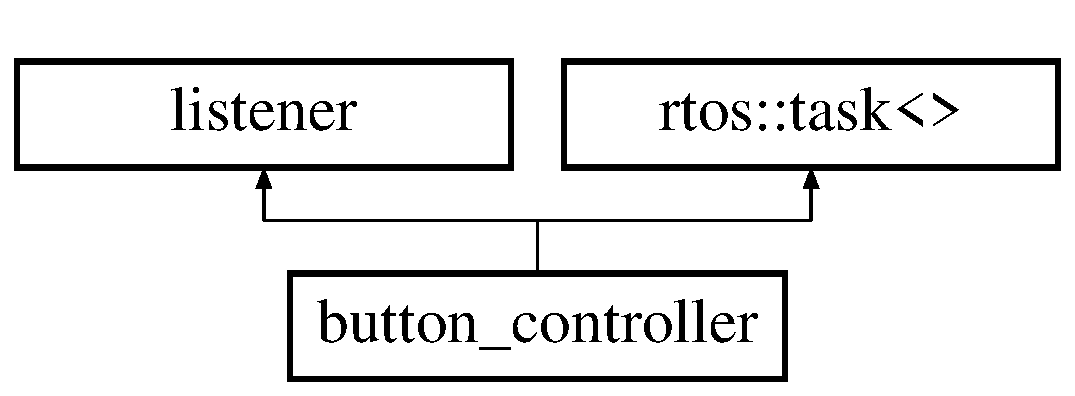
\includegraphics[height=2.000000cm]{classbutton__controller}
\end{center}
\end{figure}
\subsection*{Public Member Functions}
\begin{DoxyCompactItemize}
\item 
\hyperlink{classbutton__controller_a01cbbc0eed4933a6fe3fbf3ed565baf8}{button\+\_\+controller} (hwlib\+::pin\+\_\+in \&button\+\_\+pin, \hyperlink{classrun__game__controller}{run\+\_\+game\+\_\+controller} $\ast$run\+\_\+game)
\begin{DoxyCompactList}\small\item\em default constructor \end{DoxyCompactList}\item 
void \hyperlink{classbutton__controller_ac89e1b4894ecf3762958c97e2558d31b}{button\+\_\+pressed} () override
\begin{DoxyCompactList}\small\item\em button\+\_\+pressed \end{DoxyCompactList}\end{DoxyCompactItemize}


\subsection{Detailed Description}
\hyperlink{classbutton__controller}{button\+\_\+controller} 

This class is also a task and can be used to listen to the button. 

\subsection{Constructor \& Destructor Documentation}
\hypertarget{classbutton__controller_a01cbbc0eed4933a6fe3fbf3ed565baf8}{}\label{classbutton__controller_a01cbbc0eed4933a6fe3fbf3ed565baf8} 
\index{button\+\_\+controller@{button\+\_\+controller}!button\+\_\+controller@{button\+\_\+controller}}
\index{button\+\_\+controller@{button\+\_\+controller}!button\+\_\+controller@{button\+\_\+controller}}
\subsubsection{\texorpdfstring{button\+\_\+controller()}{button\_controller()}}
{\footnotesize\ttfamily button\+\_\+controller\+::button\+\_\+controller (\begin{DoxyParamCaption}\item[{hwlib\+::pin\+\_\+in \&}]{button\+\_\+pin,  }\item[{\hyperlink{classrun__game__controller}{run\+\_\+game\+\_\+controller} $\ast$}]{run\+\_\+game }\end{DoxyParamCaption})}



default constructor 

this constructor is used to intialize the task and the pin used for the button 

\subsection{Member Function Documentation}
\hypertarget{classbutton__controller_ac89e1b4894ecf3762958c97e2558d31b}{}\label{classbutton__controller_ac89e1b4894ecf3762958c97e2558d31b} 
\index{button\+\_\+controller@{button\+\_\+controller}!button\+\_\+pressed@{button\+\_\+pressed}}
\index{button\+\_\+pressed@{button\+\_\+pressed}!button\+\_\+controller@{button\+\_\+controller}}
\subsubsection{\texorpdfstring{button\+\_\+pressed()}{button\_pressed()}}
{\footnotesize\ttfamily void button\+\_\+controller\+::button\+\_\+pressed (\begin{DoxyParamCaption}{ }\end{DoxyParamCaption})\hspace{0.3cm}{\ttfamily [override]}, {\ttfamily [virtual]}}



button\+\_\+pressed 

this method gives functionality to the button. This method is called when the button is pressed. When the button is pressed the button sets the flag in run\+\_\+game 

Implements \hyperlink{classlistener_a22d7490fe1dce838b165d912f8015f0a}{listener}.



The documentation for this class was generated from the following files\+:\begin{DoxyCompactItemize}
\item 
\hyperlink{listenerpattern_8hpp}{listenerpattern.\+hpp}\item 
listenerpattern.\+cpp\end{DoxyCompactItemize}

\hypertarget{classgame__information__data}{}\section{game\+\_\+information\+\_\+data Class Reference}
\label{classgame__information__data}\index{game\+\_\+information\+\_\+data@{game\+\_\+information\+\_\+data}}


Store game information.  




{\ttfamily \#include $<$entity\+\_\+classes.\+hpp$>$}

\subsection*{Public Member Functions}
\begin{DoxyCompactItemize}
\item 
\hyperlink{classgame__information__data_adf5e84fd74e3e18b71b4acdc74de6844}{game\+\_\+information\+\_\+data} ()
\begin{DoxyCompactList}\small\item\em Default constructor. \end{DoxyCompactList}\item 
int \hyperlink{classgame__information__data_ad63a9f9e72242aa68cef64d53ce52249}{get\+\_\+game\+\_\+time} ()
\begin{DoxyCompactList}\small\item\em get game time \end{DoxyCompactList}\item 
bool \hyperlink{classgame__information__data_a513ec296585aedfedfd917528f9f8fe6}{get\+\_\+game\+\_\+has\+\_\+start} ()
\begin{DoxyCompactList}\small\item\em get game has started \end{DoxyCompactList}\item 
int \hyperlink{classgame__information__data_a534bcb8f2bec244ec6ab3eb200f4e301}{get\+\_\+cooldown\+\_\+time} ()
\begin{DoxyCompactList}\small\item\em get cooldown time \end{DoxyCompactList}\item 
void \hyperlink{classgame__information__data_a641a08d61da5a638cb7fe78b9c71cb11}{set\+\_\+game\+\_\+time} (int time)
\begin{DoxyCompactList}\small\item\em Set game time. \end{DoxyCompactList}\item 
void \hyperlink{classgame__information__data_a4dbb7c0d6ba269942ba417c800c66c11}{set\+\_\+game\+\_\+has\+\_\+start} (bool yes\+\_\+no)
\begin{DoxyCompactList}\small\item\em Set game has started. \end{DoxyCompactList}\item 
void \hyperlink{classgame__information__data_ab690a619ee210b5660017d8a57ed630a}{set\+\_\+cooldown\+\_\+time} (int time)
\begin{DoxyCompactList}\small\item\em Set cooldown time. \end{DoxyCompactList}\end{DoxyCompactItemize}


\subsection{Detailed Description}
Store game information. 

This entity class is used to store all the game parameters. This includes the cooldown time , the game time and a check for other objects to see if the game has started. 

\subsection{Constructor \& Destructor Documentation}
\hypertarget{classgame__information__data_adf5e84fd74e3e18b71b4acdc74de6844}{}\label{classgame__information__data_adf5e84fd74e3e18b71b4acdc74de6844} 
\index{game\+\_\+information\+\_\+data@{game\+\_\+information\+\_\+data}!game\+\_\+information\+\_\+data@{game\+\_\+information\+\_\+data}}
\index{game\+\_\+information\+\_\+data@{game\+\_\+information\+\_\+data}!game\+\_\+information\+\_\+data@{game\+\_\+information\+\_\+data}}
\subsubsection{\texorpdfstring{game\+\_\+information\+\_\+data()}{game\_information\_data()}}
{\footnotesize\ttfamily game\+\_\+information\+\_\+data\+::game\+\_\+information\+\_\+data (\begin{DoxyParamCaption}{ }\end{DoxyParamCaption})\hspace{0.3cm}{\ttfamily [inline]}}



Default constructor. 

This constructor zero initializes all data in this entity class. It dus not require any parameters. 

\subsection{Member Function Documentation}
\hypertarget{classgame__information__data_a534bcb8f2bec244ec6ab3eb200f4e301}{}\label{classgame__information__data_a534bcb8f2bec244ec6ab3eb200f4e301} 
\index{game\+\_\+information\+\_\+data@{game\+\_\+information\+\_\+data}!get\+\_\+cooldown\+\_\+time@{get\+\_\+cooldown\+\_\+time}}
\index{get\+\_\+cooldown\+\_\+time@{get\+\_\+cooldown\+\_\+time}!game\+\_\+information\+\_\+data@{game\+\_\+information\+\_\+data}}
\subsubsection{\texorpdfstring{get\+\_\+cooldown\+\_\+time()}{get\_cooldown\_time()}}
{\footnotesize\ttfamily int game\+\_\+information\+\_\+data\+::get\+\_\+cooldown\+\_\+time (\begin{DoxyParamCaption}{ }\end{DoxyParamCaption})\hspace{0.3cm}{\ttfamily [inline]}}



get cooldown time 

Gives other objects access to the private variable cooldown time. It dus not require any parameters. \hypertarget{classgame__information__data_a513ec296585aedfedfd917528f9f8fe6}{}\label{classgame__information__data_a513ec296585aedfedfd917528f9f8fe6} 
\index{game\+\_\+information\+\_\+data@{game\+\_\+information\+\_\+data}!get\+\_\+game\+\_\+has\+\_\+start@{get\+\_\+game\+\_\+has\+\_\+start}}
\index{get\+\_\+game\+\_\+has\+\_\+start@{get\+\_\+game\+\_\+has\+\_\+start}!game\+\_\+information\+\_\+data@{game\+\_\+information\+\_\+data}}
\subsubsection{\texorpdfstring{get\+\_\+game\+\_\+has\+\_\+start()}{get\_game\_has\_start()}}
{\footnotesize\ttfamily bool game\+\_\+information\+\_\+data\+::get\+\_\+game\+\_\+has\+\_\+start (\begin{DoxyParamCaption}{ }\end{DoxyParamCaption})\hspace{0.3cm}{\ttfamily [inline]}}



get game has started 

Gives other objects access to the private variable game started. It dus not require any parameters. \hypertarget{classgame__information__data_ad63a9f9e72242aa68cef64d53ce52249}{}\label{classgame__information__data_ad63a9f9e72242aa68cef64d53ce52249} 
\index{game\+\_\+information\+\_\+data@{game\+\_\+information\+\_\+data}!get\+\_\+game\+\_\+time@{get\+\_\+game\+\_\+time}}
\index{get\+\_\+game\+\_\+time@{get\+\_\+game\+\_\+time}!game\+\_\+information\+\_\+data@{game\+\_\+information\+\_\+data}}
\subsubsection{\texorpdfstring{get\+\_\+game\+\_\+time()}{get\_game\_time()}}
{\footnotesize\ttfamily int game\+\_\+information\+\_\+data\+::get\+\_\+game\+\_\+time (\begin{DoxyParamCaption}{ }\end{DoxyParamCaption})\hspace{0.3cm}{\ttfamily [inline]}}



get game time 

Gives other objects access to the private variable game\+\_\+time. Returns the game time. It dus not require any parameters. \hypertarget{classgame__information__data_ab690a619ee210b5660017d8a57ed630a}{}\label{classgame__information__data_ab690a619ee210b5660017d8a57ed630a} 
\index{game\+\_\+information\+\_\+data@{game\+\_\+information\+\_\+data}!set\+\_\+cooldown\+\_\+time@{set\+\_\+cooldown\+\_\+time}}
\index{set\+\_\+cooldown\+\_\+time@{set\+\_\+cooldown\+\_\+time}!game\+\_\+information\+\_\+data@{game\+\_\+information\+\_\+data}}
\subsubsection{\texorpdfstring{set\+\_\+cooldown\+\_\+time()}{set\_cooldown\_time()}}
{\footnotesize\ttfamily void game\+\_\+information\+\_\+data\+::set\+\_\+cooldown\+\_\+time (\begin{DoxyParamCaption}\item[{int}]{time }\end{DoxyParamCaption})\hspace{0.3cm}{\ttfamily [inline]}}



Set cooldown time. 

This function is used to set the cooldown time. It requires a integer value and dus not return anything. \hypertarget{classgame__information__data_a4dbb7c0d6ba269942ba417c800c66c11}{}\label{classgame__information__data_a4dbb7c0d6ba269942ba417c800c66c11} 
\index{game\+\_\+information\+\_\+data@{game\+\_\+information\+\_\+data}!set\+\_\+game\+\_\+has\+\_\+start@{set\+\_\+game\+\_\+has\+\_\+start}}
\index{set\+\_\+game\+\_\+has\+\_\+start@{set\+\_\+game\+\_\+has\+\_\+start}!game\+\_\+information\+\_\+data@{game\+\_\+information\+\_\+data}}
\subsubsection{\texorpdfstring{set\+\_\+game\+\_\+has\+\_\+start()}{set\_game\_has\_start()}}
{\footnotesize\ttfamily void game\+\_\+information\+\_\+data\+::set\+\_\+game\+\_\+has\+\_\+start (\begin{DoxyParamCaption}\item[{bool}]{yes\+\_\+no }\end{DoxyParamCaption})\hspace{0.3cm}{\ttfamily [inline]}}



Set game has started. 

This function is used to set the game has started variable. It requires a boolean value and dus not return anything. \hypertarget{classgame__information__data_a641a08d61da5a638cb7fe78b9c71cb11}{}\label{classgame__information__data_a641a08d61da5a638cb7fe78b9c71cb11} 
\index{game\+\_\+information\+\_\+data@{game\+\_\+information\+\_\+data}!set\+\_\+game\+\_\+time@{set\+\_\+game\+\_\+time}}
\index{set\+\_\+game\+\_\+time@{set\+\_\+game\+\_\+time}!game\+\_\+information\+\_\+data@{game\+\_\+information\+\_\+data}}
\subsubsection{\texorpdfstring{set\+\_\+game\+\_\+time()}{set\_game\_time()}}
{\footnotesize\ttfamily void game\+\_\+information\+\_\+data\+::set\+\_\+game\+\_\+time (\begin{DoxyParamCaption}\item[{int}]{time }\end{DoxyParamCaption})\hspace{0.3cm}{\ttfamily [inline]}}



Set game time. 

This function is used to set the game time. It requires a integer value and dus not return anything. 

The documentation for this class was generated from the following file\+:\begin{DoxyCompactItemize}
\item 
\hyperlink{entity__classes_8hpp}{entity\+\_\+classes.\+hpp}\end{DoxyCompactItemize}

\hypertarget{classgame__time__controller}{}\section{game\+\_\+time\+\_\+controller Class Reference}
\label{classgame__time__controller}\index{game\+\_\+time\+\_\+controller@{game\+\_\+time\+\_\+controller}}


Game time controller.  




{\ttfamily \#include $<$game\+\_\+time\+\_\+classes.\+hpp$>$}

Inheritance diagram for game\+\_\+time\+\_\+controller\+:\begin{figure}[H]
\begin{center}
\leavevmode
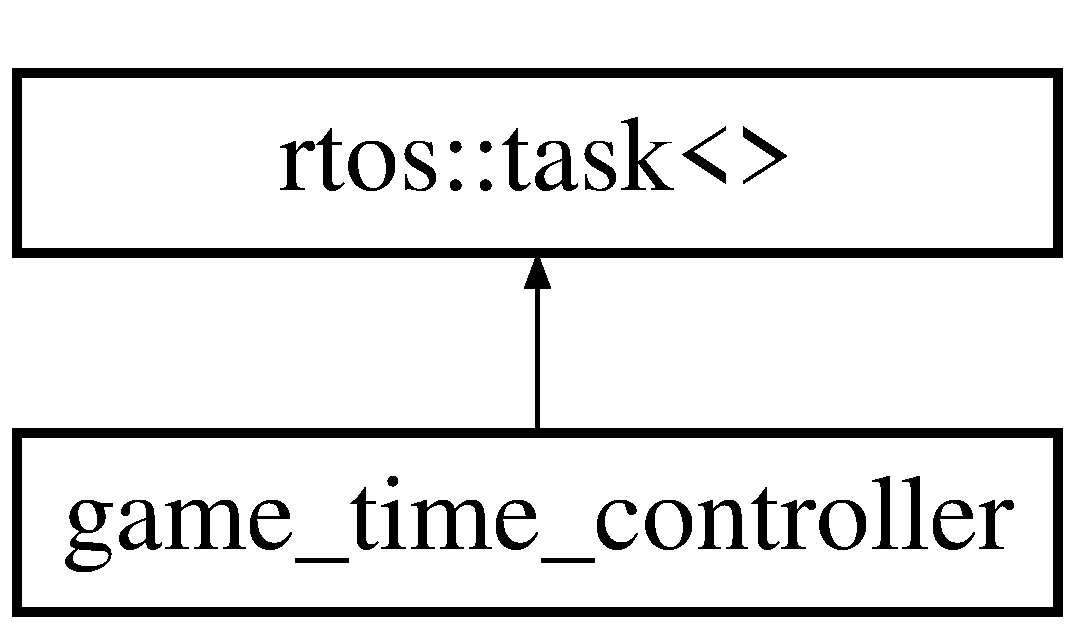
\includegraphics[height=2.000000cm]{classgame__time__controller}
\end{center}
\end{figure}
\subsection*{Public Member Functions}
\begin{DoxyCompactItemize}
\item 
\hyperlink{classgame__time__controller_ad2a906f75a90ca5c906aeb8093ac579b}{game\+\_\+time\+\_\+controller} (const char $\ast$task\+\_\+name, rtos\+::mutex \&lcd\+\_\+mutex, \hyperlink{classlcd__display__controller}{lcd\+\_\+display\+\_\+controller} \&lcd\+\_\+controller, rtos\+::flag \&game\+\_\+over\+\_\+flag)
\begin{DoxyCompactList}\small\item\em Default constructor. \end{DoxyCompactList}\item 
void \hyperlink{classgame__time__controller_a33a1f1c002465109b1caacedbf1a820f}{enable\+\_\+start\+\_\+flag} ()
\begin{DoxyCompactList}\small\item\em Enable the start flag. \end{DoxyCompactList}\item 
void \hyperlink{classgame__time__controller_a01ace9e573244e15cd28c074792b52f6}{set\+\_\+time} (int cooldown\+\_\+time, int game\+\_\+time)
\begin{DoxyCompactList}\small\item\em Set the time parameters. \end{DoxyCompactList}\end{DoxyCompactItemize}


\subsection{Detailed Description}
Game time controller. 

The game time controller is used to update the game time and display int on the lcd using the lcd\+\_\+controller. It uses a rtos clock to update the time and a flag to get it to know when to start counting. It writes the information to the game information data entity. It also receives a flag to tell when the time is over and it is the end of the game. 

\subsection{Constructor \& Destructor Documentation}
\hypertarget{classgame__time__controller_ad2a906f75a90ca5c906aeb8093ac579b}{}\label{classgame__time__controller_ad2a906f75a90ca5c906aeb8093ac579b} 
\index{game\+\_\+time\+\_\+controller@{game\+\_\+time\+\_\+controller}!game\+\_\+time\+\_\+controller@{game\+\_\+time\+\_\+controller}}
\index{game\+\_\+time\+\_\+controller@{game\+\_\+time\+\_\+controller}!game\+\_\+time\+\_\+controller@{game\+\_\+time\+\_\+controller}}
\subsubsection{\texorpdfstring{game\+\_\+time\+\_\+controller()}{game\_time\_controller()}}
{\footnotesize\ttfamily game\+\_\+time\+\_\+controller\+::game\+\_\+time\+\_\+controller (\begin{DoxyParamCaption}\item[{const char $\ast$}]{task\+\_\+name,  }\item[{rtos\+::mutex \&}]{lcd\+\_\+mutex,  }\item[{\hyperlink{classlcd__display__controller}{lcd\+\_\+display\+\_\+controller} \&}]{lcd\+\_\+controller,  }\item[{rtos\+::flag \&}]{game\+\_\+over\+\_\+flag }\end{DoxyParamCaption})\hspace{0.3cm}{\ttfamily [inline]}}



Default constructor. 

In the constructor it receives a task name, the lcd mutex, the lcd controller and the game time flag as parameters. It initializes these variables along with the flag and clock. 

\subsection{Member Function Documentation}
\hypertarget{classgame__time__controller_a33a1f1c002465109b1caacedbf1a820f}{}\label{classgame__time__controller_a33a1f1c002465109b1caacedbf1a820f} 
\index{game\+\_\+time\+\_\+controller@{game\+\_\+time\+\_\+controller}!enable\+\_\+start\+\_\+flag@{enable\+\_\+start\+\_\+flag}}
\index{enable\+\_\+start\+\_\+flag@{enable\+\_\+start\+\_\+flag}!game\+\_\+time\+\_\+controller@{game\+\_\+time\+\_\+controller}}
\subsubsection{\texorpdfstring{enable\+\_\+start\+\_\+flag()}{enable\_start\_flag()}}
{\footnotesize\ttfamily void game\+\_\+time\+\_\+controller\+::enable\+\_\+start\+\_\+flag (\begin{DoxyParamCaption}{ }\end{DoxyParamCaption})\hspace{0.3cm}{\ttfamily [inline]}}



Enable the start flag. 

This function gives other objects the ability so set the start flag. \hypertarget{classgame__time__controller_a01ace9e573244e15cd28c074792b52f6}{}\label{classgame__time__controller_a01ace9e573244e15cd28c074792b52f6} 
\index{game\+\_\+time\+\_\+controller@{game\+\_\+time\+\_\+controller}!set\+\_\+time@{set\+\_\+time}}
\index{set\+\_\+time@{set\+\_\+time}!game\+\_\+time\+\_\+controller@{game\+\_\+time\+\_\+controller}}
\subsubsection{\texorpdfstring{set\+\_\+time()}{set\_time()}}
{\footnotesize\ttfamily void game\+\_\+time\+\_\+controller\+::set\+\_\+time (\begin{DoxyParamCaption}\item[{int}]{cooldown\+\_\+time,  }\item[{int}]{game\+\_\+time }\end{DoxyParamCaption})\hspace{0.3cm}{\ttfamily [inline]}}



Set the time parameters. 

This function sets the time parameters for the game. These are created by another class. It puts these parameters into the time data entity object. The function returns nothing but dus require 2 parameters, the cooldown time and the game time. 

The documentation for this class was generated from the following file\+:\begin{DoxyCompactItemize}
\item 
\hyperlink{game__time__classes_8hpp}{game\+\_\+time\+\_\+classes.\+hpp}\end{DoxyCompactItemize}

\hypertarget{classhit}{}\section{hit Class Reference}
\label{classhit}\index{hit@{hit}}


Store a hit.  




{\ttfamily \#include $<$entity\+\_\+classes.\+hpp$>$}

\subsection*{Public Member Functions}
\begin{DoxyCompactItemize}
\item 
\hyperlink{classhit_a28033534baf49ea09fecf630e0bc9eb5}{hit} (byte player\+\_\+id, byte weapon\+\_\+id)
\begin{DoxyCompactList}\small\item\em Default constructor. \end{DoxyCompactList}\item 
byte \hyperlink{classhit_a914b4442560954de4de27f85f6168919}{get\+\_\+player\+\_\+id} ()
\begin{DoxyCompactList}\small\item\em get player id \end{DoxyCompactList}\item 
byte \hyperlink{classhit_afba4878708b2c56bddf39cfb90c1a4d9}{get\+\_\+weapon\+\_\+id} ()
\begin{DoxyCompactList}\small\item\em get weapon id \end{DoxyCompactList}\end{DoxyCompactItemize}


\subsection{Detailed Description}
Store a hit. 

Used to store hits made by other players on you. This data is beeing stored to be used to display on a computer for competitive matches. The received player id and weapon id are beeing stored. 

\subsection{Constructor \& Destructor Documentation}
\hypertarget{classhit_a28033534baf49ea09fecf630e0bc9eb5}{}\label{classhit_a28033534baf49ea09fecf630e0bc9eb5} 
\index{hit@{hit}!hit@{hit}}
\index{hit@{hit}!hit@{hit}}
\subsubsection{\texorpdfstring{hit()}{hit()}}
{\footnotesize\ttfamily hit\+::hit (\begin{DoxyParamCaption}\item[{byte}]{player\+\_\+id,  }\item[{byte}]{weapon\+\_\+id }\end{DoxyParamCaption})\hspace{0.3cm}{\ttfamily [inline]}}



Default constructor. 

The constructor initializes the player id and weapon id. These are given to the constructor as parameters. 

\subsection{Member Function Documentation}
\hypertarget{classhit_a914b4442560954de4de27f85f6168919}{}\label{classhit_a914b4442560954de4de27f85f6168919} 
\index{hit@{hit}!get\+\_\+player\+\_\+id@{get\+\_\+player\+\_\+id}}
\index{get\+\_\+player\+\_\+id@{get\+\_\+player\+\_\+id}!hit@{hit}}
\subsubsection{\texorpdfstring{get\+\_\+player\+\_\+id()}{get\_player\_id()}}
{\footnotesize\ttfamily byte hit\+::get\+\_\+player\+\_\+id (\begin{DoxyParamCaption}{ }\end{DoxyParamCaption})\hspace{0.3cm}{\ttfamily [inline]}}



get player id 

Gives other objects access to the private variable player\+\_\+id. It dus not require any parameters. \hypertarget{classhit_afba4878708b2c56bddf39cfb90c1a4d9}{}\label{classhit_afba4878708b2c56bddf39cfb90c1a4d9} 
\index{hit@{hit}!get\+\_\+weapon\+\_\+id@{get\+\_\+weapon\+\_\+id}}
\index{get\+\_\+weapon\+\_\+id@{get\+\_\+weapon\+\_\+id}!hit@{hit}}
\subsubsection{\texorpdfstring{get\+\_\+weapon\+\_\+id()}{get\_weapon\_id()}}
{\footnotesize\ttfamily byte hit\+::get\+\_\+weapon\+\_\+id (\begin{DoxyParamCaption}{ }\end{DoxyParamCaption})\hspace{0.3cm}{\ttfamily [inline]}}



get weapon id 

Gives other objects access to the private variable weapon\+\_\+id. It dus not require any parameters. 

The documentation for this class was generated from the following file\+:\begin{DoxyCompactItemize}
\item 
\hyperlink{entity__classes_8hpp}{entity\+\_\+classes.\+hpp}\end{DoxyCompactItemize}

\hypertarget{classinit__game__controller}{}\section{init\+\_\+game\+\_\+controller Class Reference}
\label{classinit__game__controller}\index{init\+\_\+game\+\_\+controller@{init\+\_\+game\+\_\+controller}}


Inialize the game.  




{\ttfamily \#include $<$init\+\_\+game.\+hpp$>$}

Inheritance diagram for init\+\_\+game\+\_\+controller\+:\begin{figure}[H]
\begin{center}
\leavevmode
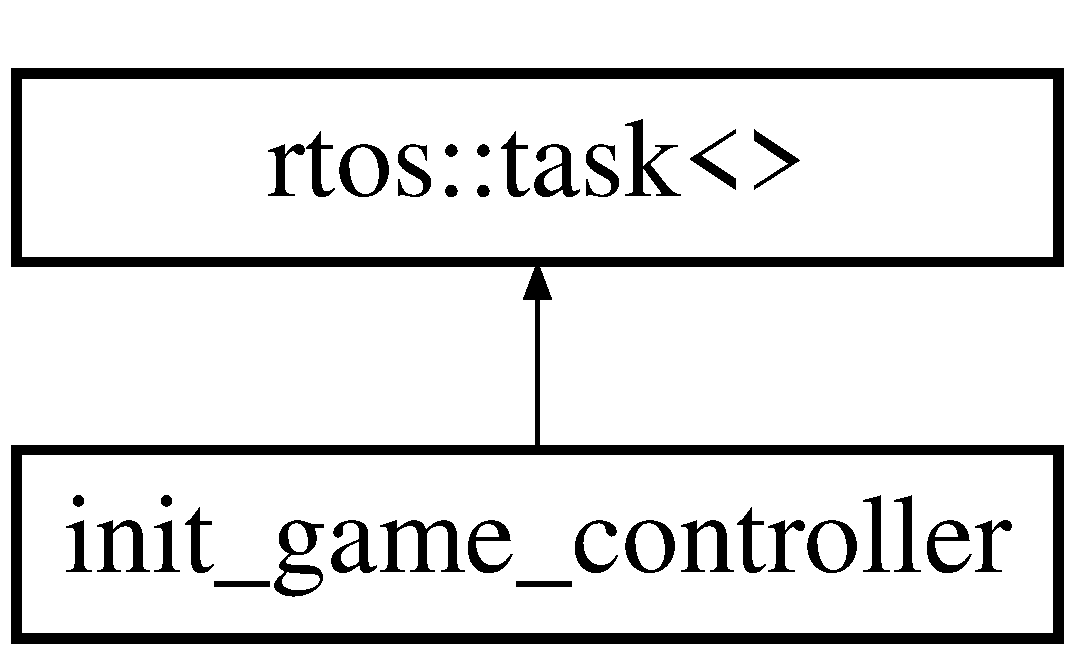
\includegraphics[height=2.000000cm]{classinit__game__controller}
\end{center}
\end{figure}
\subsection*{Public Member Functions}
\begin{DoxyCompactItemize}
\item 
\hyperlink{classinit__game__controller_a8b506bc4f98428bbceca83027a41f184}{init\+\_\+game\+\_\+controller} (\hyperlink{classlcd__display__controller}{lcd\+\_\+display\+\_\+controller} \&lcd\+\_\+controller, rtos\+::mutex \&lcd\+\_\+mutex, \hyperlink{classir__message__logic}{ir\+\_\+message\+\_\+logic} \&message)
\begin{DoxyCompactList}\small\item\em Default constructor. \end{DoxyCompactList}\end{DoxyCompactItemize}


\subsection{Detailed Description}
Inialize the game. 

This class is used for the game leader to setup the game. So far the only command the receiver expects is the game time at the beginning of the game. New commands can be added later and would need a change in the run game class. Right now during the game the receiver only exprects player ids and weapon ids but no commands. 

\subsection{Constructor \& Destructor Documentation}
\hypertarget{classinit__game__controller_a8b506bc4f98428bbceca83027a41f184}{}\label{classinit__game__controller_a8b506bc4f98428bbceca83027a41f184} 
\index{init\+\_\+game\+\_\+controller@{init\+\_\+game\+\_\+controller}!init\+\_\+game\+\_\+controller@{init\+\_\+game\+\_\+controller}}
\index{init\+\_\+game\+\_\+controller@{init\+\_\+game\+\_\+controller}!init\+\_\+game\+\_\+controller@{init\+\_\+game\+\_\+controller}}
\subsubsection{\texorpdfstring{init\+\_\+game\+\_\+controller()}{init\_game\_controller()}}
{\footnotesize\ttfamily init\+\_\+game\+\_\+controller\+::init\+\_\+game\+\_\+controller (\begin{DoxyParamCaption}\item[{\hyperlink{classlcd__display__controller}{lcd\+\_\+display\+\_\+controller} \&}]{lcd\+\_\+controller,  }\item[{rtos\+::mutex \&}]{lcd\+\_\+mutex,  }\item[{\hyperlink{classir__message__logic}{ir\+\_\+message\+\_\+logic} \&}]{message }\end{DoxyParamCaption})\hspace{0.3cm}{\ttfamily [inline]}}



Default constructor. 

This constructor receives a reference to the lcd controller and the lcd mutex. These are used to communicate with the lcds pool. The message object is there for encoding every seperate command. 

The documentation for this class was generated from the following file\+:\begin{DoxyCompactItemize}
\item 
\hyperlink{init__game_8hpp}{init\+\_\+game.\+hpp}\end{DoxyCompactItemize}

\hypertarget{classir__message__logic}{}\section{ir\+\_\+message\+\_\+logic Class Reference}
\label{classir__message__logic}\index{ir\+\_\+message\+\_\+logic@{ir\+\_\+message\+\_\+logic}}


Ir message logic class.  




{\ttfamily \#include $<$application\+\_\+logic\+\_\+classes.\+hpp$>$}

\subsection*{Public Member Functions}
\begin{DoxyCompactItemize}
\item 
\hyperlink{classir__message__logic_af65240d9b8999fd1b956fc2da17a6d3e}{ir\+\_\+message\+\_\+logic} ()
\begin{DoxyCompactList}\small\item\em Default constructor. \end{DoxyCompactList}\item 
char16\+\_\+t \hyperlink{classir__message__logic_a60cf2eae7b2ff8285440068b6419863c}{encode} (uint\+\_\+fast8\+\_\+t player\+\_\+id, uint\+\_\+fast8\+\_\+t weapon\+\_\+id)
\begin{DoxyCompactList}\small\item\em Encode ir messages. \end{DoxyCompactList}\item 
bool \hyperlink{classir__message__logic_aab003c06594ef0dd7caf33d0c928b11b}{decode} (char16\+\_\+t receiving\+\_\+bits, byte \&received\+\_\+player\+\_\+id, byte \&received\+\_\+weapon\+\_\+id)
\begin{DoxyCompactList}\small\item\em Decode the bitstream. \end{DoxyCompactList}\end{DoxyCompactItemize}


\subsection{Detailed Description}
Ir message logic class. 

This class contains all the calculations needed for the ir messages. 

\subsection{Constructor \& Destructor Documentation}
\hypertarget{classir__message__logic_af65240d9b8999fd1b956fc2da17a6d3e}{}\label{classir__message__logic_af65240d9b8999fd1b956fc2da17a6d3e} 
\index{ir\+\_\+message\+\_\+logic@{ir\+\_\+message\+\_\+logic}!ir\+\_\+message\+\_\+logic@{ir\+\_\+message\+\_\+logic}}
\index{ir\+\_\+message\+\_\+logic@{ir\+\_\+message\+\_\+logic}!ir\+\_\+message\+\_\+logic@{ir\+\_\+message\+\_\+logic}}
\subsubsection{\texorpdfstring{ir\+\_\+message\+\_\+logic()}{ir\_message\_logic()}}
{\footnotesize\ttfamily ir\+\_\+message\+\_\+logic\+::ir\+\_\+message\+\_\+logic (\begin{DoxyParamCaption}{ }\end{DoxyParamCaption})\hspace{0.3cm}{\ttfamily [inline]}}



Default constructor. 

The constructor dus not need any parameters nor dus it initialize anything. It is just there to create an object from this class. 

\subsection{Member Function Documentation}
\hypertarget{classir__message__logic_aab003c06594ef0dd7caf33d0c928b11b}{}\label{classir__message__logic_aab003c06594ef0dd7caf33d0c928b11b} 
\index{ir\+\_\+message\+\_\+logic@{ir\+\_\+message\+\_\+logic}!decode@{decode}}
\index{decode@{decode}!ir\+\_\+message\+\_\+logic@{ir\+\_\+message\+\_\+logic}}
\subsubsection{\texorpdfstring{decode()}{decode()}}
{\footnotesize\ttfamily bool ir\+\_\+message\+\_\+logic\+::decode (\begin{DoxyParamCaption}\item[{char16\+\_\+t}]{receiving\+\_\+bits,  }\item[{byte \&}]{received\+\_\+player\+\_\+id,  }\item[{byte \&}]{received\+\_\+weapon\+\_\+id }\end{DoxyParamCaption})\hspace{0.3cm}{\ttfamily [inline]}}



Decode the bitstream. 

This function decodes the bitstream in the way specified in the protocol part of the casus. It also checks the bitstream with an exor to make sure it is authentic. The function needs the bitstream as a parameter and returns zero or one depending on the result of the exor. One being exor correct and zero exor incorrect. \hypertarget{classir__message__logic_a60cf2eae7b2ff8285440068b6419863c}{}\label{classir__message__logic_a60cf2eae7b2ff8285440068b6419863c} 
\index{ir\+\_\+message\+\_\+logic@{ir\+\_\+message\+\_\+logic}!encode@{encode}}
\index{encode@{encode}!ir\+\_\+message\+\_\+logic@{ir\+\_\+message\+\_\+logic}}
\subsubsection{\texorpdfstring{encode()}{encode()}}
{\footnotesize\ttfamily char16\+\_\+t ir\+\_\+message\+\_\+logic\+::encode (\begin{DoxyParamCaption}\item[{uint\+\_\+fast8\+\_\+t}]{player\+\_\+id,  }\item[{uint\+\_\+fast8\+\_\+t}]{weapon\+\_\+id }\end{DoxyParamCaption})\hspace{0.3cm}{\ttfamily [inline]}}



Encode ir messages. 

This function is used to compile a char16\+\_\+t code that is going to be send by the ir led. The function requires two eight bit integer values and returns the char16\+\_\+t code it compiled. The code consists of a start bit. then five bits for the player id. After that 5 bits for the weapon id or for commands. Lastly the last five bits are for the exor check bits. 

The documentation for this class was generated from the following file\+:\begin{DoxyCompactItemize}
\item 
\hyperlink{application__logic__classes_8hpp}{application\+\_\+logic\+\_\+classes.\+hpp}\end{DoxyCompactItemize}

\hypertarget{classir__receiver__controller}{}\section{ir\+\_\+receiver\+\_\+controller Class Reference}
\label{classir__receiver__controller}\index{ir\+\_\+receiver\+\_\+controller@{ir\+\_\+receiver\+\_\+controller}}


\hyperlink{classir__receiver__controller}{ir\+\_\+receiver\+\_\+controller}  




{\ttfamily \#include $<$ir\+\_\+receiver\+\_\+classes.\+hpp$>$}

Inheritance diagram for ir\+\_\+receiver\+\_\+controller\+:\begin{figure}[H]
\begin{center}
\leavevmode
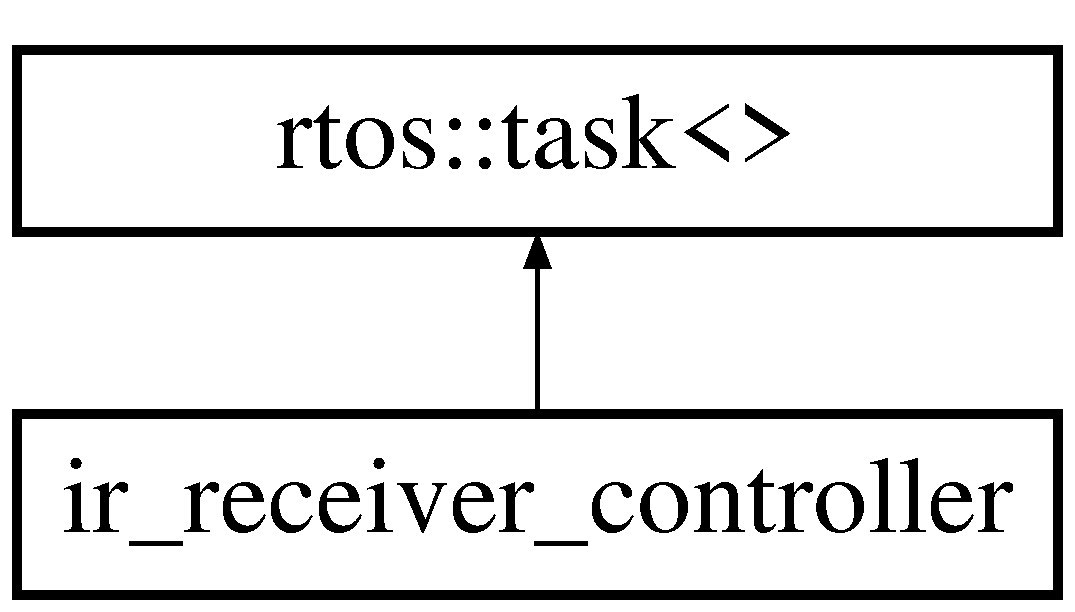
\includegraphics[height=2.000000cm]{classir__receiver__controller}
\end{center}
\end{figure}
\subsection*{Public Member Functions}
\begin{DoxyCompactItemize}
\item 
\hyperlink{classir__receiver__controller_a8ef3a05bd1d4c8531e11d57af8519146}{ir\+\_\+receiver\+\_\+controller} (hwlib\+::pin\+\_\+in \&r\+\_\+pin, hwlib\+::pin\+\_\+out \&gnd, hwlib\+::pin\+\_\+out \&vcc, \hyperlink{classrun__game__controller}{run\+\_\+game\+\_\+controller} \&run\+\_\+game)
\begin{DoxyCompactList}\small\item\em \hyperlink{classir__receiver__controller}{ir\+\_\+receiver\+\_\+controller} \end{DoxyCompactList}\item 
int \hyperlink{classir__receiver__controller_ad98b3cc0cb528a0b40e52d900638f3ec}{get\+\_\+start\+\_\+bit} ()
\begin{DoxyCompactList}\small\item\em get\+\_\+start\+\_\+bit \end{DoxyCompactList}\item 
int \hyperlink{classir__receiver__controller_a6cc44257482f6e2f463714f7b9c3784a}{get\+\_\+bit} ()
\begin{DoxyCompactList}\small\item\em Get bit. \end{DoxyCompactList}\item 
char16\+\_\+t \hyperlink{classir__receiver__controller_aaef8491c3e15d003898a4f2bfb2069d6}{get\+\_\+message} ()
\begin{DoxyCompactList}\small\item\em get\+\_\+message \end{DoxyCompactList}\end{DoxyCompactItemize}


\subsection{Detailed Description}
\hyperlink{classir__receiver__controller}{ir\+\_\+receiver\+\_\+controller} 

This class is the ir receiver class. It is a boundary object and controller object in one because we needed rtos functionality. The class uses a timer to check the ir receiver periodically. 

\subsection{Constructor \& Destructor Documentation}
\hypertarget{classir__receiver__controller_a8ef3a05bd1d4c8531e11d57af8519146}{}\label{classir__receiver__controller_a8ef3a05bd1d4c8531e11d57af8519146} 
\index{ir\+\_\+receiver\+\_\+controller@{ir\+\_\+receiver\+\_\+controller}!ir\+\_\+receiver\+\_\+controller@{ir\+\_\+receiver\+\_\+controller}}
\index{ir\+\_\+receiver\+\_\+controller@{ir\+\_\+receiver\+\_\+controller}!ir\+\_\+receiver\+\_\+controller@{ir\+\_\+receiver\+\_\+controller}}
\subsubsection{\texorpdfstring{ir\+\_\+receiver\+\_\+controller()}{ir\_receiver\_controller()}}
{\footnotesize\ttfamily ir\+\_\+receiver\+\_\+controller\+::ir\+\_\+receiver\+\_\+controller (\begin{DoxyParamCaption}\item[{hwlib\+::pin\+\_\+in \&}]{r\+\_\+pin,  }\item[{hwlib\+::pin\+\_\+out \&}]{gnd,  }\item[{hwlib\+::pin\+\_\+out \&}]{vcc,  }\item[{\hyperlink{classrun__game__controller}{run\+\_\+game\+\_\+controller} \&}]{run\+\_\+game }\end{DoxyParamCaption})\hspace{0.3cm}{\ttfamily [inline]}}



\hyperlink{classir__receiver__controller}{ir\+\_\+receiver\+\_\+controller} 

Parameters\+: one input pin, two output pins to define the ir\+\_\+receiver object. The constructor initializes the timer and all the pins. The run game controller is also initialized for use with the channel. Inside the body the ground and vcc are set. 

\subsection{Member Function Documentation}
\hypertarget{classir__receiver__controller_a6cc44257482f6e2f463714f7b9c3784a}{}\label{classir__receiver__controller_a6cc44257482f6e2f463714f7b9c3784a} 
\index{ir\+\_\+receiver\+\_\+controller@{ir\+\_\+receiver\+\_\+controller}!get\+\_\+bit@{get\+\_\+bit}}
\index{get\+\_\+bit@{get\+\_\+bit}!ir\+\_\+receiver\+\_\+controller@{ir\+\_\+receiver\+\_\+controller}}
\subsubsection{\texorpdfstring{get\+\_\+bit()}{get\_bit()}}
{\footnotesize\ttfamily int ir\+\_\+receiver\+\_\+controller\+::get\+\_\+bit (\begin{DoxyParamCaption}{ }\end{DoxyParamCaption})\hspace{0.3cm}{\ttfamily [inline]}}



Get bit. 

This function is used to get bits from the receiver. If receiving the one takes to long ($>$ 4000 us) the function will return -\/1 as an integer. The function dus not need any parameters. \hypertarget{classir__receiver__controller_aaef8491c3e15d003898a4f2bfb2069d6}{}\label{classir__receiver__controller_aaef8491c3e15d003898a4f2bfb2069d6} 
\index{ir\+\_\+receiver\+\_\+controller@{ir\+\_\+receiver\+\_\+controller}!get\+\_\+message@{get\+\_\+message}}
\index{get\+\_\+message@{get\+\_\+message}!ir\+\_\+receiver\+\_\+controller@{ir\+\_\+receiver\+\_\+controller}}
\subsubsection{\texorpdfstring{get\+\_\+message()}{get\_message()}}
{\footnotesize\ttfamily char16\+\_\+t ir\+\_\+receiver\+\_\+controller\+::get\+\_\+message (\begin{DoxyParamCaption}{ }\end{DoxyParamCaption})\hspace{0.3cm}{\ttfamily [inline]}}



get\+\_\+message 

This method is used to receive the whole message. This method can only be called after the start\+\_\+bit is received. Return value\+: char16\+\_\+t number that represent the message. The function dus not need any parameters. \hypertarget{classir__receiver__controller_ad98b3cc0cb528a0b40e52d900638f3ec}{}\label{classir__receiver__controller_ad98b3cc0cb528a0b40e52d900638f3ec} 
\index{ir\+\_\+receiver\+\_\+controller@{ir\+\_\+receiver\+\_\+controller}!get\+\_\+start\+\_\+bit@{get\+\_\+start\+\_\+bit}}
\index{get\+\_\+start\+\_\+bit@{get\+\_\+start\+\_\+bit}!ir\+\_\+receiver\+\_\+controller@{ir\+\_\+receiver\+\_\+controller}}
\subsubsection{\texorpdfstring{get\+\_\+start\+\_\+bit()}{get\_start\_bit()}}
{\footnotesize\ttfamily int ir\+\_\+receiver\+\_\+controller\+::get\+\_\+start\+\_\+bit (\begin{DoxyParamCaption}{ }\end{DoxyParamCaption})\hspace{0.3cm}{\ttfamily [inline]}}



get\+\_\+start\+\_\+bit 

This method is used to receive the first bit of a message Return value\+: This function returns a 1 or 0 depending on the value of the bit send. If there is no bit send it returns -\/1. 

The documentation for this class was generated from the following file\+:\begin{DoxyCompactItemize}
\item 
\hyperlink{ir__receiver__classes_8hpp}{ir\+\_\+receiver\+\_\+classes.\+hpp}\end{DoxyCompactItemize}

\hypertarget{classir__sender}{}\section{ir\+\_\+sender Class Reference}
\label{classir__sender}\index{ir\+\_\+sender@{ir\+\_\+sender}}


Ir sender class.  




{\ttfamily \#include $<$send\+\_\+ir\+\_\+classes.\+hpp$>$}

\subsection*{Public Member Functions}
\begin{DoxyCompactItemize}
\item 
void \hyperlink{classir__sender_a53efa5b083ddbbc9f8de912a44135e08}{send\+\_\+one} ()
\begin{DoxyCompactList}\small\item\em Send one over pin. \end{DoxyCompactList}\item 
void \hyperlink{classir__sender_a3868a2512035b0f6b5b6df093db22fbb}{send\+\_\+zero} ()
\begin{DoxyCompactList}\small\item\em Send zero over pin. \end{DoxyCompactList}\item 
void \hyperlink{classir__sender_aa38f450682d96d47347dceefb7167976}{set\+\_\+zero} ()
\begin{DoxyCompactList}\small\item\em Turn sender pin off. \end{DoxyCompactList}\item 
void \hyperlink{classir__sender_a6b23d2e93be4f000ca689395613ea487}{send\+\_\+message} (char16\+\_\+t compiled\+\_\+message)
\begin{DoxyCompactList}\small\item\em Send a full message. \end{DoxyCompactList}\item 
void \hyperlink{classir__sender_a53efa5b083ddbbc9f8de912a44135e08}{send\+\_\+one} ()
\begin{DoxyCompactList}\small\item\em Send one over pin. \end{DoxyCompactList}\item 
void \hyperlink{classir__sender_a3868a2512035b0f6b5b6df093db22fbb}{send\+\_\+zero} ()
\begin{DoxyCompactList}\small\item\em Send zero over pin. \end{DoxyCompactList}\item 
void \hyperlink{classir__sender_aa38f450682d96d47347dceefb7167976}{set\+\_\+zero} ()
\begin{DoxyCompactList}\small\item\em Turn sender pin off. \end{DoxyCompactList}\item 
void \hyperlink{classir__sender_a6b23d2e93be4f000ca689395613ea487}{send\+\_\+message} (char16\+\_\+t compiled\+\_\+message)
\begin{DoxyCompactList}\small\item\em Send a full message. \end{DoxyCompactList}\end{DoxyCompactItemize}


\subsection{Detailed Description}
Ir sender class. 

This class is a boundary object and is used to send bits in the way specified in the protocal. It contains a 36khz pin wich is arduino pin digital 2. 

\subsection{Member Function Documentation}
\hypertarget{classir__sender_a6b23d2e93be4f000ca689395613ea487}{}\label{classir__sender_a6b23d2e93be4f000ca689395613ea487} 
\index{ir\+\_\+sender@{ir\+\_\+sender}!send\+\_\+message@{send\+\_\+message}}
\index{send\+\_\+message@{send\+\_\+message}!ir\+\_\+sender@{ir\+\_\+sender}}
\subsubsection{\texorpdfstring{send\+\_\+message()}{send\_message()}\hspace{0.1cm}{\footnotesize\ttfamily [1/2]}}
{\footnotesize\ttfamily void ir\+\_\+sender\+::send\+\_\+message (\begin{DoxyParamCaption}\item[{char16\+\_\+t}]{compiled\+\_\+message }\end{DoxyParamCaption})\hspace{0.3cm}{\ttfamily [inline]}}



Send a full message. 

This function sends the complete 16 bit message. It receives the message as paramter and returns nothing. \hypertarget{classir__sender_a6b23d2e93be4f000ca689395613ea487}{}\label{classir__sender_a6b23d2e93be4f000ca689395613ea487} 
\index{ir\+\_\+sender@{ir\+\_\+sender}!send\+\_\+message@{send\+\_\+message}}
\index{send\+\_\+message@{send\+\_\+message}!ir\+\_\+sender@{ir\+\_\+sender}}
\subsubsection{\texorpdfstring{send\+\_\+message()}{send\_message()}\hspace{0.1cm}{\footnotesize\ttfamily [2/2]}}
{\footnotesize\ttfamily void ir\+\_\+sender\+::send\+\_\+message (\begin{DoxyParamCaption}\item[{char16\+\_\+t}]{compiled\+\_\+message }\end{DoxyParamCaption})\hspace{0.3cm}{\ttfamily [inline]}}



Send a full message. 

This function sends the complete 16 bit message. It receives the message as paramter and returns nothing. \hypertarget{classir__sender_a53efa5b083ddbbc9f8de912a44135e08}{}\label{classir__sender_a53efa5b083ddbbc9f8de912a44135e08} 
\index{ir\+\_\+sender@{ir\+\_\+sender}!send\+\_\+one@{send\+\_\+one}}
\index{send\+\_\+one@{send\+\_\+one}!ir\+\_\+sender@{ir\+\_\+sender}}
\subsubsection{\texorpdfstring{send\+\_\+one()}{send\_one()}\hspace{0.1cm}{\footnotesize\ttfamily [1/2]}}
{\footnotesize\ttfamily void ir\+\_\+sender\+::send\+\_\+one (\begin{DoxyParamCaption}{ }\end{DoxyParamCaption})\hspace{0.3cm}{\ttfamily [inline]}}



Send one over pin. 

This function sends a one over the sender pin. It returns nothing and dus not requires any parameters. \hypertarget{classir__sender_a53efa5b083ddbbc9f8de912a44135e08}{}\label{classir__sender_a53efa5b083ddbbc9f8de912a44135e08} 
\index{ir\+\_\+sender@{ir\+\_\+sender}!send\+\_\+one@{send\+\_\+one}}
\index{send\+\_\+one@{send\+\_\+one}!ir\+\_\+sender@{ir\+\_\+sender}}
\subsubsection{\texorpdfstring{send\+\_\+one()}{send\_one()}\hspace{0.1cm}{\footnotesize\ttfamily [2/2]}}
{\footnotesize\ttfamily void ir\+\_\+sender\+::send\+\_\+one (\begin{DoxyParamCaption}{ }\end{DoxyParamCaption})\hspace{0.3cm}{\ttfamily [inline]}}



Send one over pin. 

This function sends a one over the sender pin. It returns nothing and dus not requires any parameters. \hypertarget{classir__sender_a3868a2512035b0f6b5b6df093db22fbb}{}\label{classir__sender_a3868a2512035b0f6b5b6df093db22fbb} 
\index{ir\+\_\+sender@{ir\+\_\+sender}!send\+\_\+zero@{send\+\_\+zero}}
\index{send\+\_\+zero@{send\+\_\+zero}!ir\+\_\+sender@{ir\+\_\+sender}}
\subsubsection{\texorpdfstring{send\+\_\+zero()}{send\_zero()}\hspace{0.1cm}{\footnotesize\ttfamily [1/2]}}
{\footnotesize\ttfamily void ir\+\_\+sender\+::send\+\_\+zero (\begin{DoxyParamCaption}{ }\end{DoxyParamCaption})\hspace{0.3cm}{\ttfamily [inline]}}



Send zero over pin. 

This function sends a zero over the sender pin. It returns nothing and dus not requires any parameters. \hypertarget{classir__sender_a3868a2512035b0f6b5b6df093db22fbb}{}\label{classir__sender_a3868a2512035b0f6b5b6df093db22fbb} 
\index{ir\+\_\+sender@{ir\+\_\+sender}!send\+\_\+zero@{send\+\_\+zero}}
\index{send\+\_\+zero@{send\+\_\+zero}!ir\+\_\+sender@{ir\+\_\+sender}}
\subsubsection{\texorpdfstring{send\+\_\+zero()}{send\_zero()}\hspace{0.1cm}{\footnotesize\ttfamily [2/2]}}
{\footnotesize\ttfamily void ir\+\_\+sender\+::send\+\_\+zero (\begin{DoxyParamCaption}{ }\end{DoxyParamCaption})\hspace{0.3cm}{\ttfamily [inline]}}



Send zero over pin. 

This function sends a zero over the sender pin. It returns nothing and dus not requires any parameters. \hypertarget{classir__sender_aa38f450682d96d47347dceefb7167976}{}\label{classir__sender_aa38f450682d96d47347dceefb7167976} 
\index{ir\+\_\+sender@{ir\+\_\+sender}!set\+\_\+zero@{set\+\_\+zero}}
\index{set\+\_\+zero@{set\+\_\+zero}!ir\+\_\+sender@{ir\+\_\+sender}}
\subsubsection{\texorpdfstring{set\+\_\+zero()}{set\_zero()}\hspace{0.1cm}{\footnotesize\ttfamily [1/2]}}
{\footnotesize\ttfamily void ir\+\_\+sender\+::set\+\_\+zero (\begin{DoxyParamCaption}{ }\end{DoxyParamCaption})\hspace{0.3cm}{\ttfamily [inline]}}



Turn sender pin off. 

This function sets the sender pin to zero. It dus not need any parameters nor dus it return anything. \hypertarget{classir__sender_aa38f450682d96d47347dceefb7167976}{}\label{classir__sender_aa38f450682d96d47347dceefb7167976} 
\index{ir\+\_\+sender@{ir\+\_\+sender}!set\+\_\+zero@{set\+\_\+zero}}
\index{set\+\_\+zero@{set\+\_\+zero}!ir\+\_\+sender@{ir\+\_\+sender}}
\subsubsection{\texorpdfstring{set\+\_\+zero()}{set\_zero()}\hspace{0.1cm}{\footnotesize\ttfamily [2/2]}}
{\footnotesize\ttfamily void ir\+\_\+sender\+::set\+\_\+zero (\begin{DoxyParamCaption}{ }\end{DoxyParamCaption})\hspace{0.3cm}{\ttfamily [inline]}}



Turn sender pin off. 

This function sets the sender pin to zero. It dus not need any parameters nor dus it return anything. 

The documentation for this class was generated from the following file\+:\begin{DoxyCompactItemize}
\item 
ir sender with channel/\hyperlink{ir_01sender_01with_01channel_2send__ir__classes_8hpp}{send\+\_\+ir\+\_\+classes.\+hpp}\end{DoxyCompactItemize}

\hypertarget{class_keypad}{}\section{Keypad Class Reference}
\label{class_keypad}\index{Keypad@{Keypad}}


\hyperlink{class_keypad}{Keypad} class.  




{\ttfamily \#include $<$keypad\+\_\+class.\+hpp$>$}

\subsection*{Public Member Functions}
\begin{DoxyCompactItemize}
\item 
\hyperlink{class_keypad_a5d8b8cf0e33463dabefd8b30ec4c43e8}{Keypad} (hwlib\+::port\+\_\+oc\+\_\+from\+\_\+pins \&out\+\_\+port, hwlib\+::port\+\_\+in\+\_\+from\+\_\+pins \&in\+\_\+port)
\begin{DoxyCompactList}\small\item\em Default constructor. \end{DoxyCompactList}\item 
char \hyperlink{class_keypad_aef896a8cccb21f0b49579ed6d3c7e026}{get\+\_\+char} ()
\begin{DoxyCompactList}\small\item\em Check for input. \end{DoxyCompactList}\end{DoxyCompactItemize}


\subsection{Detailed Description}
\hyperlink{class_keypad}{Keypad} class. 

This class is an boundary object and creates a keypad from two sets of ports. 

\subsection{Constructor \& Destructor Documentation}
\hypertarget{class_keypad_a5d8b8cf0e33463dabefd8b30ec4c43e8}{}\label{class_keypad_a5d8b8cf0e33463dabefd8b30ec4c43e8} 
\index{Keypad@{Keypad}!Keypad@{Keypad}}
\index{Keypad@{Keypad}!Keypad@{Keypad}}
\subsubsection{\texorpdfstring{Keypad()}{Keypad()}}
{\footnotesize\ttfamily Keypad\+::\+Keypad (\begin{DoxyParamCaption}\item[{hwlib\+::port\+\_\+oc\+\_\+from\+\_\+pins \&}]{out\+\_\+port,  }\item[{hwlib\+::port\+\_\+in\+\_\+from\+\_\+pins \&}]{in\+\_\+port }\end{DoxyParamCaption})\hspace{0.3cm}{\ttfamily [inline]}}



Default constructor. 

This constructor receives 2 parameters. Both of them are ports created from the keypad pins. The constructor uses these ports to create a keypad. 

\subsection{Member Function Documentation}
\hypertarget{class_keypad_aef896a8cccb21f0b49579ed6d3c7e026}{}\label{class_keypad_aef896a8cccb21f0b49579ed6d3c7e026} 
\index{Keypad@{Keypad}!get\+\_\+char@{get\+\_\+char}}
\index{get\+\_\+char@{get\+\_\+char}!Keypad@{Keypad}}
\subsubsection{\texorpdfstring{get\+\_\+char()}{get\_char()}}
{\footnotesize\ttfamily char Keypad\+::get\+\_\+char (\begin{DoxyParamCaption}{ }\end{DoxyParamCaption})\hspace{0.3cm}{\ttfamily [inline]}}



Check for input. 

This function calls the getc() function from the keypad. It requires no parameters and returns the received character. The getc() function waits until a key has been pressed in a loop. 

The documentation for this class was generated from the following file\+:\begin{DoxyCompactItemize}
\item 
\hyperlink{keypad__class_8hpp}{keypad\+\_\+class.\+hpp}\end{DoxyCompactItemize}

\hypertarget{classlcd__display}{}\section{lcd\+\_\+display Class Reference}
\label{classlcd__display}\index{lcd\+\_\+display@{lcd\+\_\+display}}


display class  




{\ttfamily \#include $<$display\+\_\+classes.\+hpp$>$}

\subsection*{Public Member Functions}
\begin{DoxyCompactItemize}
\item 
\hyperlink{classlcd__display_a381883b15868b9276823270421bb2f6f}{lcd\+\_\+display} (hwlib\+::pin\+\_\+oc \&scl, hwlib\+::pin\+\_\+oc \&sda)
\begin{DoxyCompactList}\small\item\em Default constructor. \end{DoxyCompactList}\item 
void \hyperlink{classlcd__display_a74fc3a72c343a01fdc6169158bb02200}{print\+\_\+text} (const char $\ast$string, hwlib\+::font \&f)
\begin{DoxyCompactList}\small\item\em Print text on display. \end{DoxyCompactList}\end{DoxyCompactItemize}


\subsection{Detailed Description}
display class 

This is the display boundary object we use for interfacing with the lcd. It creates an lcd using a i2c bus. 

\subsection{Constructor \& Destructor Documentation}
\hypertarget{classlcd__display_a381883b15868b9276823270421bb2f6f}{}\label{classlcd__display_a381883b15868b9276823270421bb2f6f} 
\index{lcd\+\_\+display@{lcd\+\_\+display}!lcd\+\_\+display@{lcd\+\_\+display}}
\index{lcd\+\_\+display@{lcd\+\_\+display}!lcd\+\_\+display@{lcd\+\_\+display}}
\subsubsection{\texorpdfstring{lcd\+\_\+display()}{lcd\_display()}}
{\footnotesize\ttfamily lcd\+\_\+display\+::lcd\+\_\+display (\begin{DoxyParamCaption}\item[{hwlib\+::pin\+\_\+oc \&}]{scl,  }\item[{hwlib\+::pin\+\_\+oc \&}]{sda }\end{DoxyParamCaption})\hspace{0.3cm}{\ttfamily [inline]}}



Default constructor. 

This constructor receives the scl and sda lines as parameters. It then initializes them as an i2c bus. The rest of the variables and objects are also initialized and the lcd is beeing cleared. 

\subsection{Member Function Documentation}
\hypertarget{classlcd__display_a74fc3a72c343a01fdc6169158bb02200}{}\label{classlcd__display_a74fc3a72c343a01fdc6169158bb02200} 
\index{lcd\+\_\+display@{lcd\+\_\+display}!print\+\_\+text@{print\+\_\+text}}
\index{print\+\_\+text@{print\+\_\+text}!lcd\+\_\+display@{lcd\+\_\+display}}
\subsubsection{\texorpdfstring{print\+\_\+text()}{print\_text()}}
{\footnotesize\ttfamily void lcd\+\_\+display\+::print\+\_\+text (\begin{DoxyParamCaption}\item[{const char $\ast$}]{string,  }\item[{hwlib\+::font \&}]{f }\end{DoxyParamCaption})\hspace{0.3cm}{\ttfamily [inline]}}



Print text on display. 

This function prints a character array on the lcd with a specified font. It receives both these variables as parameters. There is no return value. 

The documentation for this class was generated from the following file\+:\begin{DoxyCompactItemize}
\item 
\hyperlink{display__classes_8hpp}{display\+\_\+classes.\+hpp}\end{DoxyCompactItemize}

\hypertarget{classlcd__display__controller}{}\section{lcd\+\_\+display\+\_\+controller Class Reference}
\label{classlcd__display__controller}\index{lcd\+\_\+display\+\_\+controller@{lcd\+\_\+display\+\_\+controller}}


Display controller.  




{\ttfamily \#include $<$display\+\_\+classes.\+hpp$>$}

Inheritance diagram for lcd\+\_\+display\+\_\+controller\+:\begin{figure}[H]
\begin{center}
\leavevmode
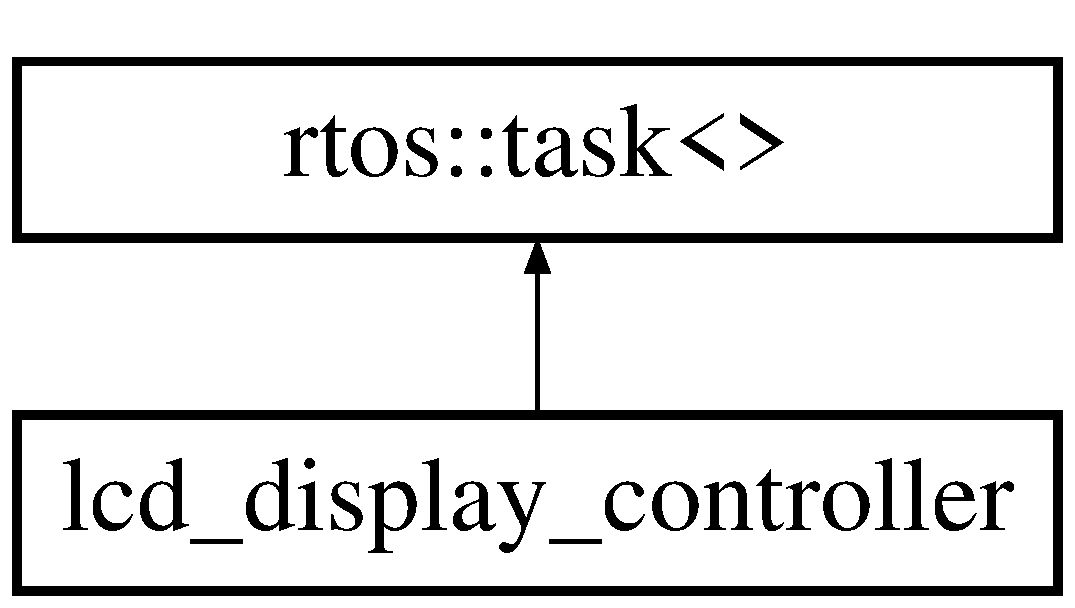
\includegraphics[height=2.000000cm]{classlcd__display__controller}
\end{center}
\end{figure}
\subsection*{Public Member Functions}
\begin{DoxyCompactItemize}
\item 
\hyperlink{classlcd__display__controller_abf42bfd4d932278f5777df103c3fd27f}{lcd\+\_\+display\+\_\+controller} (const char $\ast$task\+\_\+name, hwlib\+::pin\+\_\+oc \&scl, hwlib\+::pin\+\_\+oc \&sda, rtos\+::mutex \&lcd\+\_\+mutex)
\begin{DoxyCompactList}\small\item\em Default constructor. \end{DoxyCompactList}\item 
void \hyperlink{classlcd__display__controller_a66aacdfab1cbf14bd9cfe844fbb34b8a}{write} (const \hyperlink{structlcd__passthrough}{lcd\+\_\+passthrough} lcd\+\_\+struct)
\begin{DoxyCompactList}\small\item\em Write to pool. \end{DoxyCompactList}\item 
\hyperlink{structlcd__passthrough}{lcd\+\_\+passthrough} \hyperlink{classlcd__display__controller_a9eb5a62f4b813f0ea44b3c7efaa6ec0a}{read} ()
\begin{DoxyCompactList}\small\item\em Read from pool. \end{DoxyCompactList}\item 
void \hyperlink{classlcd__display__controller_af37be06c27c0eb1e67dbeb8e8e2df8c1}{enable\+\_\+flag} ()
\begin{DoxyCompactList}\small\item\em Enable the lcd information changed flag. \end{DoxyCompactList}\end{DoxyCompactItemize}


\subsection{Detailed Description}
Display controller. 

The display controller is used to get information to be printed from a pool with mutex and then output it on the lcd. 

\subsection{Constructor \& Destructor Documentation}
\hypertarget{classlcd__display__controller_abf42bfd4d932278f5777df103c3fd27f}{}\label{classlcd__display__controller_abf42bfd4d932278f5777df103c3fd27f} 
\index{lcd\+\_\+display\+\_\+controller@{lcd\+\_\+display\+\_\+controller}!lcd\+\_\+display\+\_\+controller@{lcd\+\_\+display\+\_\+controller}}
\index{lcd\+\_\+display\+\_\+controller@{lcd\+\_\+display\+\_\+controller}!lcd\+\_\+display\+\_\+controller@{lcd\+\_\+display\+\_\+controller}}
\subsubsection{\texorpdfstring{lcd\+\_\+display\+\_\+controller()}{lcd\_display\_controller()}}
{\footnotesize\ttfamily lcd\+\_\+display\+\_\+controller\+::lcd\+\_\+display\+\_\+controller (\begin{DoxyParamCaption}\item[{const char $\ast$}]{task\+\_\+name,  }\item[{hwlib\+::pin\+\_\+oc \&}]{scl,  }\item[{hwlib\+::pin\+\_\+oc \&}]{sda,  }\item[{rtos\+::mutex \&}]{lcd\+\_\+mutex }\end{DoxyParamCaption})\hspace{0.3cm}{\ttfamily [inline]}}



Default constructor. 

This constructor receives a task name, scl pin, sda pin, and lcd mutex as parameters. It initializes these variables and creates the oled object from them. It also initializes the information changed flag. 

\subsection{Member Function Documentation}
\hypertarget{classlcd__display__controller_af37be06c27c0eb1e67dbeb8e8e2df8c1}{}\label{classlcd__display__controller_af37be06c27c0eb1e67dbeb8e8e2df8c1} 
\index{lcd\+\_\+display\+\_\+controller@{lcd\+\_\+display\+\_\+controller}!enable\+\_\+flag@{enable\+\_\+flag}}
\index{enable\+\_\+flag@{enable\+\_\+flag}!lcd\+\_\+display\+\_\+controller@{lcd\+\_\+display\+\_\+controller}}
\subsubsection{\texorpdfstring{enable\+\_\+flag()}{enable\_flag()}}
{\footnotesize\ttfamily void lcd\+\_\+display\+\_\+controller\+::enable\+\_\+flag (\begin{DoxyParamCaption}{ }\end{DoxyParamCaption})\hspace{0.3cm}{\ttfamily [inline]}}



Enable the lcd information changed flag. 

This function is used to set the information changed flag so the main knows that new information has to be put on screen. The function dus not need any parameters nor dus it return anything. \hypertarget{classlcd__display__controller_a9eb5a62f4b813f0ea44b3c7efaa6ec0a}{}\label{classlcd__display__controller_a9eb5a62f4b813f0ea44b3c7efaa6ec0a} 
\index{lcd\+\_\+display\+\_\+controller@{lcd\+\_\+display\+\_\+controller}!read@{read}}
\index{read@{read}!lcd\+\_\+display\+\_\+controller@{lcd\+\_\+display\+\_\+controller}}
\subsubsection{\texorpdfstring{read()}{read()}}
{\footnotesize\ttfamily \hyperlink{structlcd__passthrough}{lcd\+\_\+passthrough} lcd\+\_\+display\+\_\+controller\+::read (\begin{DoxyParamCaption}{ }\end{DoxyParamCaption})\hspace{0.3cm}{\ttfamily [inline]}}



Read from pool. 

This function is used to read the current data from the pool. This makes other objects able to read the current data displayed on the lcd and change a single line while maintaining the rest of the data. It returns the information from the pool and dus not need any parameters. \hypertarget{classlcd__display__controller_a66aacdfab1cbf14bd9cfe844fbb34b8a}{}\label{classlcd__display__controller_a66aacdfab1cbf14bd9cfe844fbb34b8a} 
\index{lcd\+\_\+display\+\_\+controller@{lcd\+\_\+display\+\_\+controller}!write@{write}}
\index{write@{write}!lcd\+\_\+display\+\_\+controller@{lcd\+\_\+display\+\_\+controller}}
\subsubsection{\texorpdfstring{write()}{write()}}
{\footnotesize\ttfamily void lcd\+\_\+display\+\_\+controller\+::write (\begin{DoxyParamCaption}\item[{const \hyperlink{structlcd__passthrough}{lcd\+\_\+passthrough}}]{lcd\+\_\+struct }\end{DoxyParamCaption})\hspace{0.3cm}{\ttfamily [inline]}}



Write to pool. 

This function makes other classes able to write lcd passthrough structures to the lcd pool. It returns nothing and receives the structure to write as an parameter. 

The documentation for this class was generated from the following file\+:\begin{DoxyCompactItemize}
\item 
\hyperlink{display__classes_8hpp}{display\+\_\+classes.\+hpp}\end{DoxyCompactItemize}

\hypertarget{structlcd__passthrough}{}\section{lcd\+\_\+passthrough Struct Reference}
\label{structlcd__passthrough}\index{lcd\+\_\+passthrough@{lcd\+\_\+passthrough}}


Lcd line structure.  




{\ttfamily \#include $<$display\+\_\+classes.\+hpp$>$}

\subsection*{Public Member Functions}
\begin{DoxyCompactItemize}
\item 
void \hyperlink{structlcd__passthrough_a74c4254fef0e0e422ac0e078d7824c3a}{assignment} (char $\ast$array, const char $\ast$other)
\begin{DoxyCompactList}\small\item\em Assign character array to line. \end{DoxyCompactList}\end{DoxyCompactItemize}
\subsection*{Public Attributes}
\begin{DoxyCompactItemize}
\item 
\hypertarget{structlcd__passthrough_a33de361ffdcc3a003b317df1c7f4e931}{}\label{structlcd__passthrough_a33de361ffdcc3a003b317df1c7f4e931} 
char {\bfseries line1} \mbox{[}16\mbox{]} = \char`\"{}\char`\"{}
\item 
\hypertarget{structlcd__passthrough_a168d61fecb6e46fc814a004f28f7e64f}{}\label{structlcd__passthrough_a168d61fecb6e46fc814a004f28f7e64f} 
char {\bfseries line2} \mbox{[}16\mbox{]} = \char`\"{}\char`\"{}
\item 
\hypertarget{structlcd__passthrough_afaab03e889a8417894e5e23268969276}{}\label{structlcd__passthrough_afaab03e889a8417894e5e23268969276} 
char {\bfseries line3} \mbox{[}16\mbox{]} = \char`\"{}\char`\"{}
\item 
\hypertarget{structlcd__passthrough_a17db87a86d7232445024e336abefe4f9}{}\label{structlcd__passthrough_a17db87a86d7232445024e336abefe4f9} 
char {\bfseries line4} \mbox{[}16\mbox{]} = \char`\"{}\char`\"{}
\item 
\hypertarget{structlcd__passthrough_a79943b73fa79c1ca25b39fa1538d6cf6}{}\label{structlcd__passthrough_a79943b73fa79c1ca25b39fa1538d6cf6} 
char {\bfseries line5} \mbox{[}16\mbox{]} = \char`\"{}\char`\"{}
\item 
\hypertarget{structlcd__passthrough_a03b23e976dba9d2e5f83ed059e56b332}{}\label{structlcd__passthrough_a03b23e976dba9d2e5f83ed059e56b332} 
char {\bfseries line6} \mbox{[}16\mbox{]} = \char`\"{}\char`\"{}
\item 
\hypertarget{structlcd__passthrough_ac7d27a96a3b6c25ebc2a2539ec631e81}{}\label{structlcd__passthrough_ac7d27a96a3b6c25ebc2a2539ec631e81} 
char {\bfseries line7} \mbox{[}16\mbox{]} = \char`\"{}\char`\"{}
\item 
\hypertarget{structlcd__passthrough_a753b84809de13c39b85b2a569211eaa2}{}\label{structlcd__passthrough_a753b84809de13c39b85b2a569211eaa2} 
char {\bfseries line8} \mbox{[}16\mbox{]} = \char`\"{}\char`\"{}
\item 
\hypertarget{structlcd__passthrough_aebb53028202d32c5b94643f7ca138609}{}\label{structlcd__passthrough_aebb53028202d32c5b94643f7ca138609} 
bool {\bfseries player\+\_\+hit} = false
\item 
\hypertarget{structlcd__passthrough_a522dee420466fc4cf7c873e0db5dfccb}{}\label{structlcd__passthrough_a522dee420466fc4cf7c873e0db5dfccb} 
bool {\bfseries game\+\_\+end} = false
\item 
\hypertarget{structlcd__passthrough_a423c70d93fcc677406a38a5e7b70e874}{}\label{structlcd__passthrough_a423c70d93fcc677406a38a5e7b70e874} 
bool {\bfseries game\+\_\+begin} = false
\end{DoxyCompactItemize}


\subsection{Detailed Description}
Lcd line structure. 

This structure is used to make sure we can edit individual lines on the lcd. It contains 8 lines of 16 characters long. There are also some boolean values for making it easy to tell the controller you want one of three bigger texts on the lcd. These texts are \char`\"{}hit\char`\"{}, \char`\"{}game begin\char`\"{} and \char`\"{}game end\char`\"{} 

\subsection{Member Function Documentation}
\hypertarget{structlcd__passthrough_a74c4254fef0e0e422ac0e078d7824c3a}{}\label{structlcd__passthrough_a74c4254fef0e0e422ac0e078d7824c3a} 
\index{lcd\+\_\+passthrough@{lcd\+\_\+passthrough}!assignment@{assignment}}
\index{assignment@{assignment}!lcd\+\_\+passthrough@{lcd\+\_\+passthrough}}
\subsubsection{\texorpdfstring{assignment()}{assignment()}}
{\footnotesize\ttfamily void lcd\+\_\+passthrough\+::assignment (\begin{DoxyParamCaption}\item[{char $\ast$}]{array,  }\item[{const char $\ast$}]{other }\end{DoxyParamCaption})\hspace{0.3cm}{\ttfamily [inline]}}



Assign character array to line. 

This function is used to assign a character array to the specified line. It makes sure that two different sized character arrays can be used. The function dus not have a return value but requires two char arrays as parameters. 

The documentation for this struct was generated from the following file\+:\begin{DoxyCompactItemize}
\item 
\hyperlink{display__classes_8hpp}{display\+\_\+classes.\+hpp}\end{DoxyCompactItemize}

\hypertarget{structled__color__behaviour}{}\section{led\+\_\+color\+\_\+behaviour Struct Reference}
\label{structled__color__behaviour}\index{led\+\_\+color\+\_\+behaviour@{led\+\_\+color\+\_\+behaviour}}


Provide led color information.  




{\ttfamily \#include $<$rgb\+\_\+led\+\_\+classes.\+hpp$>$}

\subsection*{Public Attributes}
\begin{DoxyCompactItemize}
\item 
\hypertarget{structled__color__behaviour_a7b361774f3548f07e087525c2a78fe78}{}\label{structled__color__behaviour_a7b361774f3548f07e087525c2a78fe78} 
bool {\bfseries red} = false
\item 
\hypertarget{structled__color__behaviour_a35e719a7d391ab42db18595348acbdd5}{}\label{structled__color__behaviour_a35e719a7d391ab42db18595348acbdd5} 
bool {\bfseries green} = false
\item 
\hypertarget{structled__color__behaviour_acae43a677eaddda748c5bfd3a5caa75b}{}\label{structled__color__behaviour_acae43a677eaddda748c5bfd3a5caa75b} 
bool {\bfseries blue} = false
\end{DoxyCompactItemize}


\subsection{Detailed Description}
Provide led color information. 

This struct is used to provide information about what color needs to be visable on the led. 

The documentation for this struct was generated from the following file\+:\begin{DoxyCompactItemize}
\item 
\hyperlink{rgb__led__classes_8hpp}{rgb\+\_\+led\+\_\+classes.\+hpp}\end{DoxyCompactItemize}

\hypertarget{classled__controller}{}\section{led\+\_\+controller Class Reference}
\label{classled__controller}\index{led\+\_\+controller@{led\+\_\+controller}}


Led controller class.  




{\ttfamily \#include $<$rgb\+\_\+led\+\_\+classes.\+hpp$>$}

Inheritance diagram for led\+\_\+controller\+:\begin{figure}[H]
\begin{center}
\leavevmode
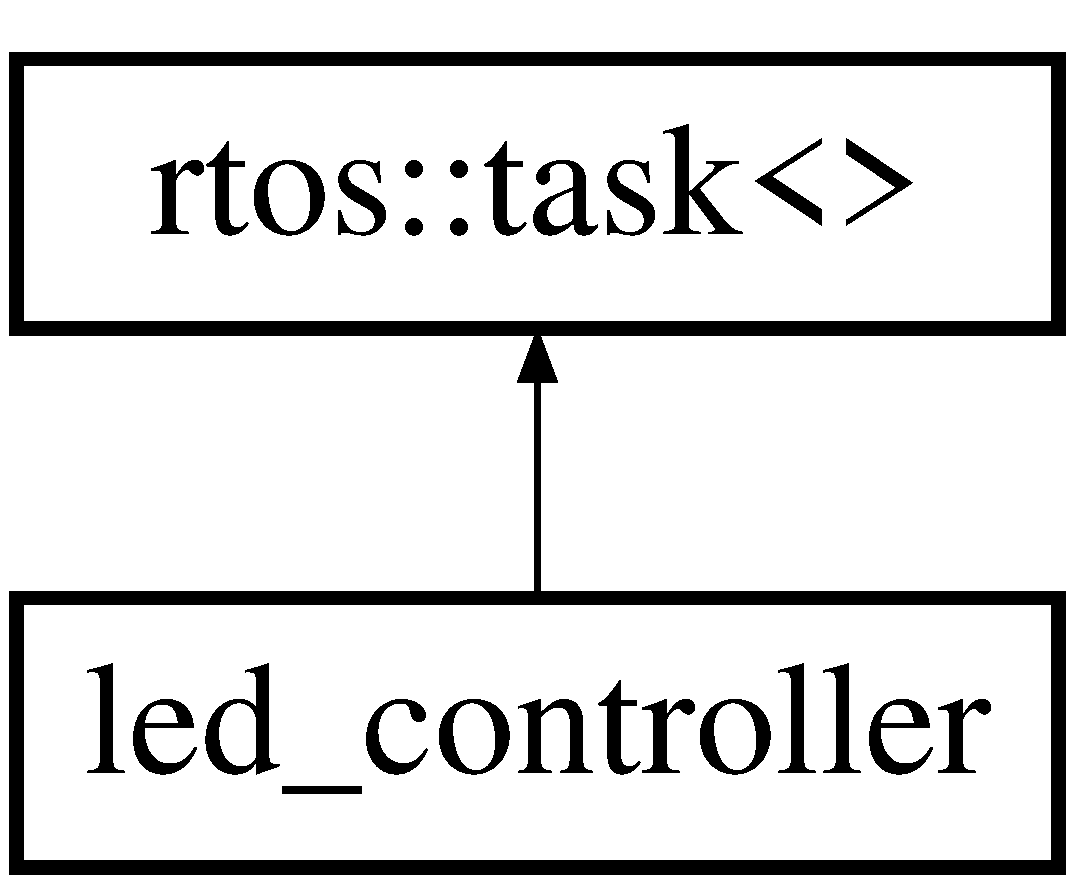
\includegraphics[height=2.000000cm]{classled__controller}
\end{center}
\end{figure}
\subsection*{Public Member Functions}
\begin{DoxyCompactItemize}
\item 
\hyperlink{classled__controller_a1ace48b14131910317e79e64df4306f5}{led\+\_\+controller} (const char $\ast$task\+\_\+name, hwlib\+::pin\+\_\+out \&r, hwlib\+::pin\+\_\+out \&g, hwlib\+::pin\+\_\+out \&b)
\begin{DoxyCompactList}\small\item\em Default constructor. \end{DoxyCompactList}\item 
void \hyperlink{classled__controller_a346241076add950fe9c929d22039e171}{write} (\hyperlink{structled__color__behaviour}{led\+\_\+color\+\_\+behaviour} color)
\begin{DoxyCompactList}\small\item\em Write to the led color channel. \end{DoxyCompactList}\end{DoxyCompactItemize}


\subsection{Detailed Description}
Led controller class. 

This class controls the behaviour of the led. It receives this behaviour through a rtos channel. 

\subsection{Constructor \& Destructor Documentation}
\hypertarget{classled__controller_a1ace48b14131910317e79e64df4306f5}{}\label{classled__controller_a1ace48b14131910317e79e64df4306f5} 
\index{led\+\_\+controller@{led\+\_\+controller}!led\+\_\+controller@{led\+\_\+controller}}
\index{led\+\_\+controller@{led\+\_\+controller}!led\+\_\+controller@{led\+\_\+controller}}
\subsubsection{\texorpdfstring{led\+\_\+controller()}{led\_controller()}}
{\footnotesize\ttfamily led\+\_\+controller\+::led\+\_\+controller (\begin{DoxyParamCaption}\item[{const char $\ast$}]{task\+\_\+name,  }\item[{hwlib\+::pin\+\_\+out \&}]{r,  }\item[{hwlib\+::pin\+\_\+out \&}]{g,  }\item[{hwlib\+::pin\+\_\+out \&}]{b }\end{DoxyParamCaption})\hspace{0.3cm}{\ttfamily [inline]}}



Default constructor. 

This constructor receives a task name and three pins. The pins from the led. The led object gets initialized with the three pins. The channel is also initialized. 

\subsection{Member Function Documentation}
\hypertarget{classled__controller_a346241076add950fe9c929d22039e171}{}\label{classled__controller_a346241076add950fe9c929d22039e171} 
\index{led\+\_\+controller@{led\+\_\+controller}!write@{write}}
\index{write@{write}!led\+\_\+controller@{led\+\_\+controller}}
\subsubsection{\texorpdfstring{write()}{write()}}
{\footnotesize\ttfamily void led\+\_\+controller\+::write (\begin{DoxyParamCaption}\item[{\hyperlink{structled__color__behaviour}{led\+\_\+color\+\_\+behaviour}}]{color }\end{DoxyParamCaption})\hspace{0.3cm}{\ttfamily [inline]}}



Write to the led color channel. 

This function makes sure other objects can write to the channel. It dus not return anything and needs a led color behaviour structure as parameter. 

The documentation for this class was generated from the following file\+:\begin{DoxyCompactItemize}
\item 
\hyperlink{rgb__led__classes_8hpp}{rgb\+\_\+led\+\_\+classes.\+hpp}\end{DoxyCompactItemize}

\hypertarget{classlistener}{}\section{listener Class Reference}
\label{classlistener}\index{listener@{listener}}


Listener.  




{\ttfamily \#include $<$listenerpattern.\+hpp$>$}

Inheritance diagram for listener\+:\begin{figure}[H]
\begin{center}
\leavevmode
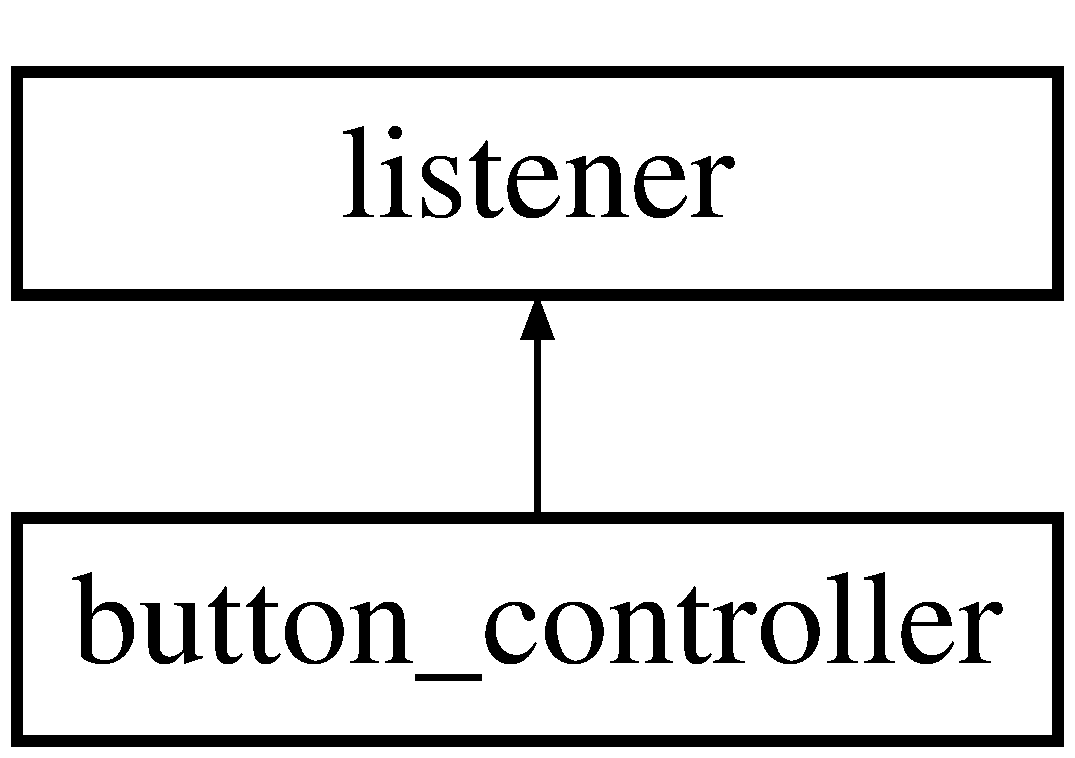
\includegraphics[height=2.000000cm]{classlistener}
\end{center}
\end{figure}
\subsection*{Public Member Functions}
\begin{DoxyCompactItemize}
\item 
virtual void \hyperlink{classlistener_a22d7490fe1dce838b165d912f8015f0a}{button\+\_\+pressed} ()=0
\begin{DoxyCompactList}\small\item\em button\+\_\+pressed \end{DoxyCompactList}\end{DoxyCompactItemize}


\subsection{Detailed Description}
Listener. 

This class is used to listen to the button 

\subsection{Member Function Documentation}
\hypertarget{classlistener_a22d7490fe1dce838b165d912f8015f0a}{}\label{classlistener_a22d7490fe1dce838b165d912f8015f0a} 
\index{listener@{listener}!button\+\_\+pressed@{button\+\_\+pressed}}
\index{button\+\_\+pressed@{button\+\_\+pressed}!listener@{listener}}
\subsubsection{\texorpdfstring{button\+\_\+pressed()}{button\_pressed()}}
{\footnotesize\ttfamily virtual void listener\+::button\+\_\+pressed (\begin{DoxyParamCaption}{ }\end{DoxyParamCaption})\hspace{0.3cm}{\ttfamily [pure virtual]}}



button\+\_\+pressed 

this method is abstract and is used by button controller 

Implemented in \hyperlink{classbutton__controller_ac89e1b4894ecf3762958c97e2558d31b}{button\+\_\+controller}.



The documentation for this class was generated from the following file\+:\begin{DoxyCompactItemize}
\item 
\hyperlink{listenerpattern_8hpp}{listenerpattern.\+hpp}\end{DoxyCompactItemize}

\hypertarget{classmy__player__information}{}\section{my\+\_\+player\+\_\+information Class Reference}
\label{classmy__player__information}\index{my\+\_\+player\+\_\+information@{my\+\_\+player\+\_\+information}}


Save the player information.  




{\ttfamily \#include $<$entity\+\_\+classes.\+hpp$>$}

\subsection*{Public Member Functions}
\begin{DoxyCompactItemize}
\item 
\hyperlink{classmy__player__information_a32ffeb6d9e2850542685e4fb40e28f9a}{my\+\_\+player\+\_\+information} ()
\begin{DoxyCompactList}\small\item\em Default constructor. \end{DoxyCompactList}\item 
char16\+\_\+t \hyperlink{classmy__player__information_a065c0e06903f41d5ecfcadbf7bd0bb12}{get\+\_\+compiled\+\_\+bits} ()
\begin{DoxyCompactList}\small\item\em get compiled bits \end{DoxyCompactList}\item 
int \hyperlink{classmy__player__information_a627d9bfc027e556998519c7ff9eff157}{get\+\_\+health} ()
\begin{DoxyCompactList}\small\item\em get player health \end{DoxyCompactList}\item 
void \hyperlink{classmy__player__information_a0cbbe520cb8591e71f1ac4164c9536d2}{set\+\_\+compiled\+\_\+bits} (char16\+\_\+t value)
\begin{DoxyCompactList}\small\item\em Set compiled bits. \end{DoxyCompactList}\item 
void \hyperlink{classmy__player__information_ae7c84c2a5a688d61f9452c78d6e8e82e}{set\+\_\+health} (int value)
\begin{DoxyCompactList}\small\item\em Set player health. \end{DoxyCompactList}\end{DoxyCompactItemize}


\subsection{Detailed Description}
Save the player information. 

This class contains the health of a player and the compiled bits that need to be send when the player shoots. 

\subsection{Constructor \& Destructor Documentation}
\hypertarget{classmy__player__information_a32ffeb6d9e2850542685e4fb40e28f9a}{}\label{classmy__player__information_a32ffeb6d9e2850542685e4fb40e28f9a} 
\index{my\+\_\+player\+\_\+information@{my\+\_\+player\+\_\+information}!my\+\_\+player\+\_\+information@{my\+\_\+player\+\_\+information}}
\index{my\+\_\+player\+\_\+information@{my\+\_\+player\+\_\+information}!my\+\_\+player\+\_\+information@{my\+\_\+player\+\_\+information}}
\subsubsection{\texorpdfstring{my\+\_\+player\+\_\+information()}{my\_player\_information()}}
{\footnotesize\ttfamily my\+\_\+player\+\_\+information\+::my\+\_\+player\+\_\+information (\begin{DoxyParamCaption}{ }\end{DoxyParamCaption})\hspace{0.3cm}{\ttfamily [inline]}}



Default constructor. 

Zero initializes the compiled bits because those will be compiled later. It also initializes the health of the player. It has no parameters. 

\subsection{Member Function Documentation}
\hypertarget{classmy__player__information_a065c0e06903f41d5ecfcadbf7bd0bb12}{}\label{classmy__player__information_a065c0e06903f41d5ecfcadbf7bd0bb12} 
\index{my\+\_\+player\+\_\+information@{my\+\_\+player\+\_\+information}!get\+\_\+compiled\+\_\+bits@{get\+\_\+compiled\+\_\+bits}}
\index{get\+\_\+compiled\+\_\+bits@{get\+\_\+compiled\+\_\+bits}!my\+\_\+player\+\_\+information@{my\+\_\+player\+\_\+information}}
\subsubsection{\texorpdfstring{get\+\_\+compiled\+\_\+bits()}{get\_compiled\_bits()}}
{\footnotesize\ttfamily char16\+\_\+t my\+\_\+player\+\_\+information\+::get\+\_\+compiled\+\_\+bits (\begin{DoxyParamCaption}{ }\end{DoxyParamCaption})\hspace{0.3cm}{\ttfamily [inline]}}



get compiled bits 

Gives other objects access to the private variable compiled bits. Returns the compiled bits. It dus not require any parameters. \hypertarget{classmy__player__information_a627d9bfc027e556998519c7ff9eff157}{}\label{classmy__player__information_a627d9bfc027e556998519c7ff9eff157} 
\index{my\+\_\+player\+\_\+information@{my\+\_\+player\+\_\+information}!get\+\_\+health@{get\+\_\+health}}
\index{get\+\_\+health@{get\+\_\+health}!my\+\_\+player\+\_\+information@{my\+\_\+player\+\_\+information}}
\subsubsection{\texorpdfstring{get\+\_\+health()}{get\_health()}}
{\footnotesize\ttfamily int my\+\_\+player\+\_\+information\+::get\+\_\+health (\begin{DoxyParamCaption}{ }\end{DoxyParamCaption})\hspace{0.3cm}{\ttfamily [inline]}}



get player health 

Gives other objects access to the private variable health. Returns the health. It dus not require any parameters. \hypertarget{classmy__player__information_a0cbbe520cb8591e71f1ac4164c9536d2}{}\label{classmy__player__information_a0cbbe520cb8591e71f1ac4164c9536d2} 
\index{my\+\_\+player\+\_\+information@{my\+\_\+player\+\_\+information}!set\+\_\+compiled\+\_\+bits@{set\+\_\+compiled\+\_\+bits}}
\index{set\+\_\+compiled\+\_\+bits@{set\+\_\+compiled\+\_\+bits}!my\+\_\+player\+\_\+information@{my\+\_\+player\+\_\+information}}
\subsubsection{\texorpdfstring{set\+\_\+compiled\+\_\+bits()}{set\_compiled\_bits()}}
{\footnotesize\ttfamily void my\+\_\+player\+\_\+information\+::set\+\_\+compiled\+\_\+bits (\begin{DoxyParamCaption}\item[{char16\+\_\+t}]{value }\end{DoxyParamCaption})\hspace{0.3cm}{\ttfamily [inline]}}



Set compiled bits. 

This function is used to set the compiled bits. It requires a char16\+\_\+t value and dus not return anything. \hypertarget{classmy__player__information_ae7c84c2a5a688d61f9452c78d6e8e82e}{}\label{classmy__player__information_ae7c84c2a5a688d61f9452c78d6e8e82e} 
\index{my\+\_\+player\+\_\+information@{my\+\_\+player\+\_\+information}!set\+\_\+health@{set\+\_\+health}}
\index{set\+\_\+health@{set\+\_\+health}!my\+\_\+player\+\_\+information@{my\+\_\+player\+\_\+information}}
\subsubsection{\texorpdfstring{set\+\_\+health()}{set\_health()}}
{\footnotesize\ttfamily void my\+\_\+player\+\_\+information\+::set\+\_\+health (\begin{DoxyParamCaption}\item[{int}]{value }\end{DoxyParamCaption})\hspace{0.3cm}{\ttfamily [inline]}}



Set player health. 

This function is used to set the player health. It requires a integer value and dus not return anything. 

The documentation for this class was generated from the following file\+:\begin{DoxyCompactItemize}
\item 
\hyperlink{entity__classes_8hpp}{entity\+\_\+classes.\+hpp}\end{DoxyCompactItemize}

\hypertarget{classregister__game__parameters__controller}{}\section{register\+\_\+game\+\_\+parameters\+\_\+controller Class Reference}
\label{classregister__game__parameters__controller}\index{register\+\_\+game\+\_\+parameters\+\_\+controller@{register\+\_\+game\+\_\+parameters\+\_\+controller}}


\hyperlink{classregister__game__parameters__controller}{register\+\_\+game\+\_\+parameters\+\_\+controller}  




{\ttfamily \#include $<$register\+\_\+game\+\_\+parameters\+\_\+class.\+hpp$>$}

\subsection*{Public Member Functions}
\begin{DoxyCompactItemize}
\item 
\hyperlink{classregister__game__parameters__controller_a291e306ca9e214208d0145058af13eeb}{register\+\_\+game\+\_\+parameters\+\_\+controller} (\hyperlink{classir__message__logic}{ir\+\_\+message\+\_\+logic} \&compile, \hyperlink{classmy__player__information}{my\+\_\+player\+\_\+information} \&information, \hyperlink{class_keypad}{Keypad} \&keypad)
\begin{DoxyCompactList}\small\item\em Default constructor. \end{DoxyCompactList}\item 
bool \hyperlink{classregister__game__parameters__controller_a9599db32b65bd0839ae4037acfdadd95}{setup} (char key)
\begin{DoxyCompactList}\small\item\em Setup function. \end{DoxyCompactList}\end{DoxyCompactItemize}


\subsection{Detailed Description}
\hyperlink{classregister__game__parameters__controller}{register\+\_\+game\+\_\+parameters\+\_\+controller} 

This class registers a player and weapon id and it encodes the message that is to be send when the player shoots. 

\subsection{Constructor \& Destructor Documentation}
\hypertarget{classregister__game__parameters__controller_a291e306ca9e214208d0145058af13eeb}{}\label{classregister__game__parameters__controller_a291e306ca9e214208d0145058af13eeb} 
\index{register\+\_\+game\+\_\+parameters\+\_\+controller@{register\+\_\+game\+\_\+parameters\+\_\+controller}!register\+\_\+game\+\_\+parameters\+\_\+controller@{register\+\_\+game\+\_\+parameters\+\_\+controller}}
\index{register\+\_\+game\+\_\+parameters\+\_\+controller@{register\+\_\+game\+\_\+parameters\+\_\+controller}!register\+\_\+game\+\_\+parameters\+\_\+controller@{register\+\_\+game\+\_\+parameters\+\_\+controller}}
\subsubsection{\texorpdfstring{register\+\_\+game\+\_\+parameters\+\_\+controller()}{register\_game\_parameters\_controller()}}
{\footnotesize\ttfamily register\+\_\+game\+\_\+parameters\+\_\+controller\+::register\+\_\+game\+\_\+parameters\+\_\+controller (\begin{DoxyParamCaption}\item[{\hyperlink{classir__message__logic}{ir\+\_\+message\+\_\+logic} \&}]{compile,  }\item[{\hyperlink{classmy__player__information}{my\+\_\+player\+\_\+information} \&}]{information,  }\item[{\hyperlink{class_keypad}{Keypad} \&}]{keypad }\end{DoxyParamCaption})\hspace{0.3cm}{\ttfamily [inline]}}



Default constructor. 

This constructor receives the ir message logic, the player information and the keypad. It receives these all by reference so the can keep on existing after the class is destructed. All other variables are zero initialized 

\subsection{Member Function Documentation}
\hypertarget{classregister__game__parameters__controller_a9599db32b65bd0839ae4037acfdadd95}{}\label{classregister__game__parameters__controller_a9599db32b65bd0839ae4037acfdadd95} 
\index{register\+\_\+game\+\_\+parameters\+\_\+controller@{register\+\_\+game\+\_\+parameters\+\_\+controller}!setup@{setup}}
\index{setup@{setup}!register\+\_\+game\+\_\+parameters\+\_\+controller@{register\+\_\+game\+\_\+parameters\+\_\+controller}}
\subsubsection{\texorpdfstring{setup()}{setup()}}
{\footnotesize\ttfamily bool register\+\_\+game\+\_\+parameters\+\_\+controller\+::setup (\begin{DoxyParamCaption}\item[{char}]{key }\end{DoxyParamCaption})\hspace{0.3cm}{\ttfamily [inline]}}



Setup function. 

This function is called from the run game class. It receives the pressed key as a parameter. After that it checks what the pressed key whas and returns a 0 if the loop in run game needs to continue and a 1 if it needs to stop. 

The documentation for this class was generated from the following file\+:\begin{DoxyCompactItemize}
\item 
\hyperlink{register__game__parameters__class_8hpp}{register\+\_\+game\+\_\+parameters\+\_\+class.\+hpp}\end{DoxyCompactItemize}

\hypertarget{classrgb__led}{}\section{rgb\+\_\+led Class Reference}
\label{classrgb__led}\index{rgb\+\_\+led@{rgb\+\_\+led}}


Rgb led.  




{\ttfamily \#include $<$rgb\+\_\+led\+\_\+classes.\+hpp$>$}

\subsection*{Public Member Functions}
\begin{DoxyCompactItemize}
\item 
\hyperlink{classrgb__led_ab8a4367c1d76a6274e65230524af0456}{rgb\+\_\+led} (hwlib\+::pin\+\_\+out \&r, hwlib\+::pin\+\_\+out \&g, hwlib\+::pin\+\_\+out \&b)
\begin{DoxyCompactList}\small\item\em Default constructor. \end{DoxyCompactList}\item 
void \hyperlink{classrgb__led_aaf7cc1181e7ddafbd199c669bd2bace1}{set\+\_\+red} ()
\begin{DoxyCompactList}\small\item\em turn the red color on \end{DoxyCompactList}\item 
void \hyperlink{classrgb__led_a1832619177bce8c5221e3495af1c081c}{set\+\_\+green} ()
\begin{DoxyCompactList}\small\item\em turn the green color on \end{DoxyCompactList}\item 
void \hyperlink{classrgb__led_acaebeada28c4603b975fe3e5f328cc8e}{set\+\_\+blue} ()
\begin{DoxyCompactList}\small\item\em turn the blue color on \end{DoxyCompactList}\item 
void \hyperlink{classrgb__led_ab22d036c95b9eaa96cd73ec33758a4f0}{off} ()
\begin{DoxyCompactList}\small\item\em turn the led of \end{DoxyCompactList}\end{DoxyCompactItemize}


\subsection{Detailed Description}
Rgb led. 

Simple boundary object used to set an rgb led to one of the three colors. 

\subsection{Constructor \& Destructor Documentation}
\hypertarget{classrgb__led_ab8a4367c1d76a6274e65230524af0456}{}\label{classrgb__led_ab8a4367c1d76a6274e65230524af0456} 
\index{rgb\+\_\+led@{rgb\+\_\+led}!rgb\+\_\+led@{rgb\+\_\+led}}
\index{rgb\+\_\+led@{rgb\+\_\+led}!rgb\+\_\+led@{rgb\+\_\+led}}
\subsubsection{\texorpdfstring{rgb\+\_\+led()}{rgb\_led()}}
{\footnotesize\ttfamily rgb\+\_\+led\+::rgb\+\_\+led (\begin{DoxyParamCaption}\item[{hwlib\+::pin\+\_\+out \&}]{r,  }\item[{hwlib\+::pin\+\_\+out \&}]{g,  }\item[{hwlib\+::pin\+\_\+out \&}]{b }\end{DoxyParamCaption})\hspace{0.3cm}{\ttfamily [inline]}}



Default constructor. 

This constructor gets three pins as parameters and initializes them. 

\subsection{Member Function Documentation}
\hypertarget{classrgb__led_ab22d036c95b9eaa96cd73ec33758a4f0}{}\label{classrgb__led_ab22d036c95b9eaa96cd73ec33758a4f0} 
\index{rgb\+\_\+led@{rgb\+\_\+led}!off@{off}}
\index{off@{off}!rgb\+\_\+led@{rgb\+\_\+led}}
\subsubsection{\texorpdfstring{off()}{off()}}
{\footnotesize\ttfamily void rgb\+\_\+led\+::off (\begin{DoxyParamCaption}{ }\end{DoxyParamCaption})\hspace{0.3cm}{\ttfamily [inline]}}



turn the led of 

This function turns off all the led colors. It dus not need any parameters nor dus it return anything. \hypertarget{classrgb__led_acaebeada28c4603b975fe3e5f328cc8e}{}\label{classrgb__led_acaebeada28c4603b975fe3e5f328cc8e} 
\index{rgb\+\_\+led@{rgb\+\_\+led}!set\+\_\+blue@{set\+\_\+blue}}
\index{set\+\_\+blue@{set\+\_\+blue}!rgb\+\_\+led@{rgb\+\_\+led}}
\subsubsection{\texorpdfstring{set\+\_\+blue()}{set\_blue()}}
{\footnotesize\ttfamily void rgb\+\_\+led\+::set\+\_\+blue (\begin{DoxyParamCaption}{ }\end{DoxyParamCaption})\hspace{0.3cm}{\ttfamily [inline]}}



turn the blue color on 

This function turns on the blue color on the led while turing off the other colors. It dus not need any parameters nor dus it return anything. \hypertarget{classrgb__led_a1832619177bce8c5221e3495af1c081c}{}\label{classrgb__led_a1832619177bce8c5221e3495af1c081c} 
\index{rgb\+\_\+led@{rgb\+\_\+led}!set\+\_\+green@{set\+\_\+green}}
\index{set\+\_\+green@{set\+\_\+green}!rgb\+\_\+led@{rgb\+\_\+led}}
\subsubsection{\texorpdfstring{set\+\_\+green()}{set\_green()}}
{\footnotesize\ttfamily void rgb\+\_\+led\+::set\+\_\+green (\begin{DoxyParamCaption}{ }\end{DoxyParamCaption})\hspace{0.3cm}{\ttfamily [inline]}}



turn the green color on 

This function turns on the green color on the led while turing off the other colors. It dus not need any parameters nor dus it return anything. \hypertarget{classrgb__led_aaf7cc1181e7ddafbd199c669bd2bace1}{}\label{classrgb__led_aaf7cc1181e7ddafbd199c669bd2bace1} 
\index{rgb\+\_\+led@{rgb\+\_\+led}!set\+\_\+red@{set\+\_\+red}}
\index{set\+\_\+red@{set\+\_\+red}!rgb\+\_\+led@{rgb\+\_\+led}}
\subsubsection{\texorpdfstring{set\+\_\+red()}{set\_red()}}
{\footnotesize\ttfamily void rgb\+\_\+led\+::set\+\_\+red (\begin{DoxyParamCaption}{ }\end{DoxyParamCaption})\hspace{0.3cm}{\ttfamily [inline]}}



turn the red color on 

This function turns on the red color on the led while turing off the other colors. It dus not need any parameters nor dus it return anything. 

The documentation for this class was generated from the following file\+:\begin{DoxyCompactItemize}
\item 
\hyperlink{rgb__led__classes_8hpp}{rgb\+\_\+led\+\_\+classes.\+hpp}\end{DoxyCompactItemize}

\hypertarget{classrun__game__controller}{}\section{run\+\_\+game\+\_\+controller Class Reference}
\label{classrun__game__controller}\index{run\+\_\+game\+\_\+controller@{run\+\_\+game\+\_\+controller}}


run the game  




{\ttfamily \#include $<$run\+\_\+game.\+hpp$>$}

Inheritance diagram for run\+\_\+game\+\_\+controller\+:\begin{figure}[H]
\begin{center}
\leavevmode
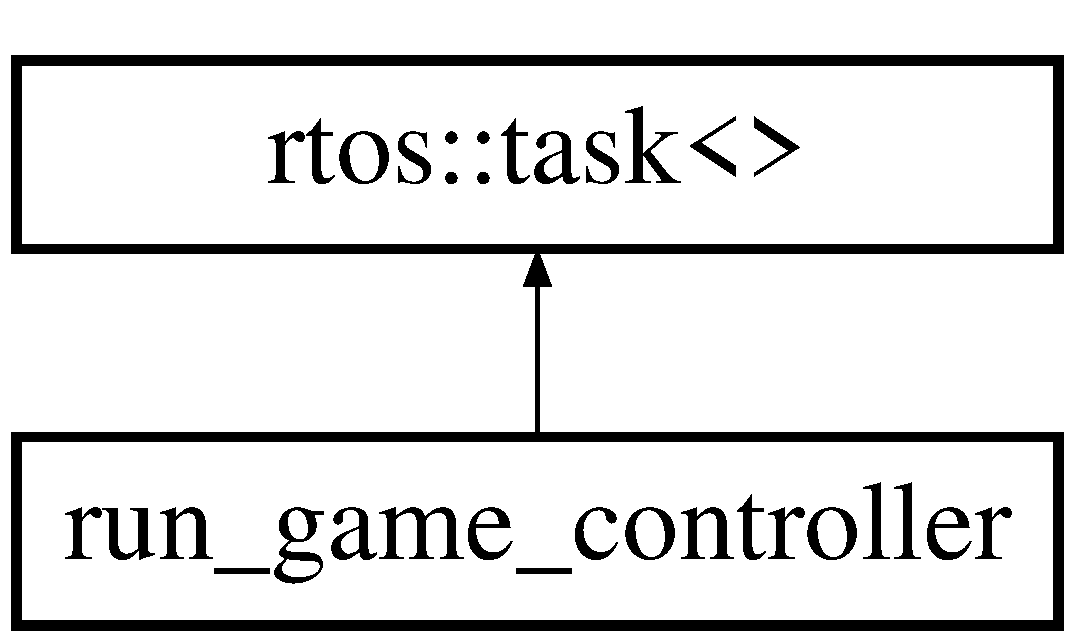
\includegraphics[height=2.000000cm]{classrun__game__controller}
\end{center}
\end{figure}
\subsection*{Public Member Functions}
\begin{DoxyCompactItemize}
\item 
\hyperlink{classrun__game__controller_aa61968bc65e1ad20a5065ccfd7d598da}{run\+\_\+game\+\_\+controller} (\hyperlink{classlcd__display__controller}{lcd\+\_\+display\+\_\+controller} \&lcd\+\_\+controller, rtos\+::mutex \&lcd\+\_\+mutex, \hyperlink{classir__message__logic}{ir\+\_\+message\+\_\+logic} \&message\+\_\+logic, \hyperlink{classmy__player__information}{my\+\_\+player\+\_\+information} \&player\+\_\+information, rtos\+::mutex \&sound\+\_\+mutex)
\begin{DoxyCompactList}\small\item\em Default constructor. \end{DoxyCompactList}\item 
void \hyperlink{classrun__game__controller_a45846159930efd40f9b20ecf72e36003}{enable\+\_\+flag} ()
\begin{DoxyCompactList}\small\item\em Enable the button flag. \end{DoxyCompactList}\item 
\hypertarget{classrun__game__controller_ae5329a8ebb79ad5021dd6eedd24f7e0e}{}\label{classrun__game__controller_ae5329a8ebb79ad5021dd6eedd24f7e0e} 
void {\bfseries write} (char16\+\_\+t value)
\end{DoxyCompactItemize}


\subsection{Detailed Description}
run the game 

This class is the total package of the game. Most of the classes used are created in this class. It coordinates almost all the information flows. 

\subsection{Constructor \& Destructor Documentation}
\hypertarget{classrun__game__controller_aa61968bc65e1ad20a5065ccfd7d598da}{}\label{classrun__game__controller_aa61968bc65e1ad20a5065ccfd7d598da} 
\index{run\+\_\+game\+\_\+controller@{run\+\_\+game\+\_\+controller}!run\+\_\+game\+\_\+controller@{run\+\_\+game\+\_\+controller}}
\index{run\+\_\+game\+\_\+controller@{run\+\_\+game\+\_\+controller}!run\+\_\+game\+\_\+controller@{run\+\_\+game\+\_\+controller}}
\subsubsection{\texorpdfstring{run\+\_\+game\+\_\+controller()}{run\_game\_controller()}}
{\footnotesize\ttfamily run\+\_\+game\+\_\+controller\+::run\+\_\+game\+\_\+controller (\begin{DoxyParamCaption}\item[{\hyperlink{classlcd__display__controller}{lcd\+\_\+display\+\_\+controller} \&}]{lcd\+\_\+controller,  }\item[{rtos\+::mutex \&}]{lcd\+\_\+mutex,  }\item[{\hyperlink{classir__message__logic}{ir\+\_\+message\+\_\+logic} \&}]{message\+\_\+logic,  }\item[{\hyperlink{classmy__player__information}{my\+\_\+player\+\_\+information} \&}]{player\+\_\+information,  }\item[{rtos\+::mutex \&}]{sound\+\_\+mutex }\end{DoxyParamCaption})\hspace{0.3cm}{\ttfamily [inline]}}



Default constructor. 

The constructor of this class initializes a lot of objects needed for the object to work. The parameters are all the parts that are created outside the class. This consists of the lcd controller object, the lcd mutex, the message application logic object, the player information entity and the sound mutex. 

\subsection{Member Function Documentation}
\hypertarget{classrun__game__controller_a45846159930efd40f9b20ecf72e36003}{}\label{classrun__game__controller_a45846159930efd40f9b20ecf72e36003} 
\index{run\+\_\+game\+\_\+controller@{run\+\_\+game\+\_\+controller}!enable\+\_\+flag@{enable\+\_\+flag}}
\index{enable\+\_\+flag@{enable\+\_\+flag}!run\+\_\+game\+\_\+controller@{run\+\_\+game\+\_\+controller}}
\subsubsection{\texorpdfstring{enable\+\_\+flag()}{enable\_flag()}}
{\footnotesize\ttfamily void run\+\_\+game\+\_\+controller\+::enable\+\_\+flag (\begin{DoxyParamCaption}{ }\end{DoxyParamCaption})\hspace{0.3cm}{\ttfamily [inline]}}



Enable the button flag. 

This function gives other objects the ability so set the button pressed flag. 

The documentation for this class was generated from the following file\+:\begin{DoxyCompactItemize}
\item 
\hyperlink{run__game_8hpp}{run\+\_\+game.\+hpp}\end{DoxyCompactItemize}

\hypertarget{classsend__controller}{}\section{send\+\_\+controller Class Reference}
\label{classsend__controller}\index{send\+\_\+controller@{send\+\_\+controller}}


Ir send controller.  




{\ttfamily \#include $<$send\+\_\+ir\+\_\+classes.\+hpp$>$}

Inheritance diagram for send\+\_\+controller\+:\begin{figure}[H]
\begin{center}
\leavevmode
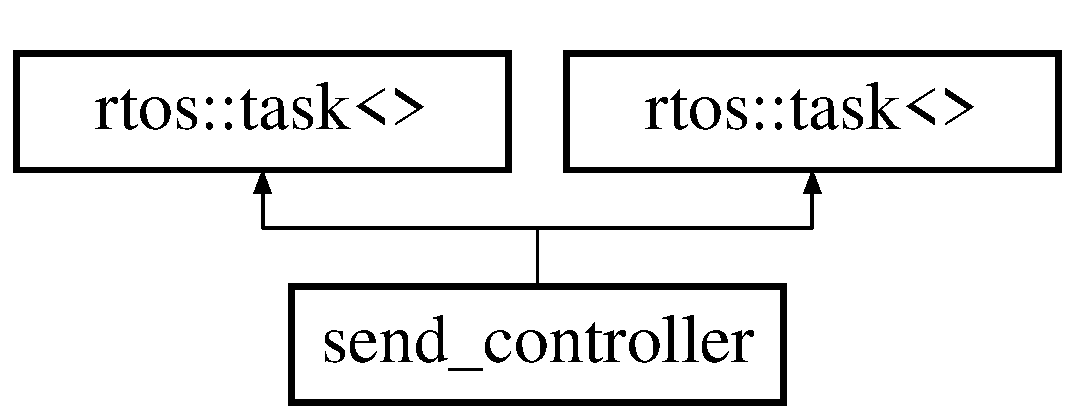
\includegraphics[height=2.000000cm]{classsend__controller}
\end{center}
\end{figure}
\subsection*{Public Member Functions}
\begin{DoxyCompactItemize}
\item 
\hyperlink{classsend__controller_a31abdb529dba4bde0893bf04d0ef113d}{send\+\_\+controller} ()
\begin{DoxyCompactList}\small\item\em Default constructor. \end{DoxyCompactList}\item 
void \hyperlink{classsend__controller_ada7d206636bf7b867696cfa8fdd080b2}{write} (char16\+\_\+t value)
\begin{DoxyCompactList}\small\item\em Write to the messages channel. \end{DoxyCompactList}\item 
\hyperlink{classsend__controller_a4f7f3b8afe7b94c3b6f284ad31fb4492}{send\+\_\+controller} (\hyperlink{classmy__player__information}{my\+\_\+player\+\_\+information} \&player\+\_\+information)
\begin{DoxyCompactList}\small\item\em Default constructor. \end{DoxyCompactList}\item 
void \hyperlink{classsend__controller_a29cfa70656efe2e26bc2c7cebe84ee46}{enable\+\_\+flag} ()
\begin{DoxyCompactList}\small\item\em Set the send message flag. \end{DoxyCompactList}\end{DoxyCompactItemize}


\subsection{Detailed Description}
Ir send controller. 

An object of this class can be created to send bits using the in the casus specified protocol. 

\subsection{Constructor \& Destructor Documentation}
\hypertarget{classsend__controller_a31abdb529dba4bde0893bf04d0ef113d}{}\label{classsend__controller_a31abdb529dba4bde0893bf04d0ef113d} 
\index{send\+\_\+controller@{send\+\_\+controller}!send\+\_\+controller@{send\+\_\+controller}}
\index{send\+\_\+controller@{send\+\_\+controller}!send\+\_\+controller@{send\+\_\+controller}}
\subsubsection{\texorpdfstring{send\+\_\+controller()}{send\_controller()}\hspace{0.1cm}{\footnotesize\ttfamily [1/2]}}
{\footnotesize\ttfamily send\+\_\+controller\+::send\+\_\+controller (\begin{DoxyParamCaption}{ }\end{DoxyParamCaption})\hspace{0.3cm}{\ttfamily [inline]}}



Default constructor. 

The constructor initializes all the objects of this class and creates a ir sender object. \hypertarget{classsend__controller_a4f7f3b8afe7b94c3b6f284ad31fb4492}{}\label{classsend__controller_a4f7f3b8afe7b94c3b6f284ad31fb4492} 
\index{send\+\_\+controller@{send\+\_\+controller}!send\+\_\+controller@{send\+\_\+controller}}
\index{send\+\_\+controller@{send\+\_\+controller}!send\+\_\+controller@{send\+\_\+controller}}
\subsubsection{\texorpdfstring{send\+\_\+controller()}{send\_controller()}\hspace{0.1cm}{\footnotesize\ttfamily [2/2]}}
{\footnotesize\ttfamily send\+\_\+controller\+::send\+\_\+controller (\begin{DoxyParamCaption}\item[{\hyperlink{classmy__player__information}{my\+\_\+player\+\_\+information} \&}]{player\+\_\+information }\end{DoxyParamCaption})\hspace{0.3cm}{\ttfamily [inline]}}



Default constructor. 

This constructor receives a reference to the player information as a parameters and initializes all the variables. 

\subsection{Member Function Documentation}
\hypertarget{classsend__controller_a29cfa70656efe2e26bc2c7cebe84ee46}{}\label{classsend__controller_a29cfa70656efe2e26bc2c7cebe84ee46} 
\index{send\+\_\+controller@{send\+\_\+controller}!enable\+\_\+flag@{enable\+\_\+flag}}
\index{enable\+\_\+flag@{enable\+\_\+flag}!send\+\_\+controller@{send\+\_\+controller}}
\subsubsection{\texorpdfstring{enable\+\_\+flag()}{enable\_flag()}}
{\footnotesize\ttfamily void send\+\_\+controller\+::enable\+\_\+flag (\begin{DoxyParamCaption}{ }\end{DoxyParamCaption})\hspace{0.3cm}{\ttfamily [inline]}}



Set the send message flag. 

This function makes other objects able to set the send message flag. \hypertarget{classsend__controller_ada7d206636bf7b867696cfa8fdd080b2}{}\label{classsend__controller_ada7d206636bf7b867696cfa8fdd080b2} 
\index{send\+\_\+controller@{send\+\_\+controller}!write@{write}}
\index{write@{write}!send\+\_\+controller@{send\+\_\+controller}}
\subsubsection{\texorpdfstring{write()}{write()}}
{\footnotesize\ttfamily void send\+\_\+controller\+::write (\begin{DoxyParamCaption}\item[{char16\+\_\+t}]{value }\end{DoxyParamCaption})\hspace{0.3cm}{\ttfamily [inline]}}



Write to the messages channel. 

This function makes other objects able to wirte char16\+\_\+t values to the messages channel. 

The documentation for this class was generated from the following file\+:\begin{DoxyCompactItemize}
\item 
ir sender with channel/\hyperlink{ir_01sender_01with_01channel_2send__ir__classes_8hpp}{send\+\_\+ir\+\_\+classes.\+hpp}\end{DoxyCompactItemize}

\hypertarget{structsound__lookup}{}\section{sound\+\_\+lookup Struct Reference}
\label{structsound__lookup}\index{sound\+\_\+lookup@{sound\+\_\+lookup}}


Data structure for sound\+\_\+storage.  




{\ttfamily \#include $<$speaker\+\_\+classes.\+hpp$>$}

\subsection*{Public Attributes}
\begin{DoxyCompactItemize}
\item 
\hypertarget{structsound__lookup_a3f597ffbf84891f44319e621db98ef81}{}\label{structsound__lookup_a3f597ffbf84891f44319e621db98ef81} 
int {\bfseries frequency}
\item 
\hypertarget{structsound__lookup_a7a155cf327d9ef451c1e9b04f940a12b}{}\label{structsound__lookup_a7a155cf327d9ef451c1e9b04f940a12b} 
int {\bfseries duration}
\item 
\hypertarget{structsound__lookup_ab6b83a017a9d6a4e28628c20f63ad473}{}\label{structsound__lookup_ab6b83a017a9d6a4e28628c20f63ad473} 
int {\bfseries amount}
\item 
\hypertarget{structsound__lookup_a8bcf50a31f32ff0081133edc380bb0a1}{}\label{structsound__lookup_a8bcf50a31f32ff0081133edc380bb0a1} 
int {\bfseries amount\+\_\+wait}
\end{DoxyCompactItemize}


\subsection{Detailed Description}
Data structure for sound\+\_\+storage. 

structure for storage of frequency, duration, amount( of tones), amount\+\_\+wait(time between tones in ms) 

The documentation for this struct was generated from the following file\+:\begin{DoxyCompactItemize}
\item 
\hyperlink{speaker__classes_8hpp}{speaker\+\_\+classes.\+hpp}\end{DoxyCompactItemize}

\hypertarget{classspeaker}{}\section{speaker Class Reference}
\label{classspeaker}\index{speaker@{speaker}}


speaker class  




{\ttfamily \#include $<$speaker\+\_\+classes.\+hpp$>$}

\subsection*{Public Member Functions}
\begin{DoxyCompactItemize}
\item 
\hyperlink{classspeaker_a3c4dcbdc5d9cc99e1fa6c30dea0235c3}{speaker} (hwlib\+::pin\+\_\+out \&speaker\+\_\+pin)
\begin{DoxyCompactList}\small\item\em Default constructor. \end{DoxyCompactList}\item 
void \hyperlink{classspeaker_a625c84e34f9ee40a7baeb2d6baa816a1}{play} (const uint\+\_\+fast16\+\_\+t frequency, const uint\+\_\+fast16\+\_\+t duration, const uint\+\_\+fast16\+\_\+t amount, const uint\+\_\+fast16\+\_\+t amount\+\_\+wait)
\begin{DoxyCompactList}\small\item\em Play function. \end{DoxyCompactList}\end{DoxyCompactItemize}


\subsection{Detailed Description}
speaker class 

Simple player class for playing frequency\textquotesingle{}s on a speaker connected to a G\+P\+IO pin. Created by Wouter van Ooijen.(modified) 

\subsection{Constructor \& Destructor Documentation}
\hypertarget{classspeaker_a3c4dcbdc5d9cc99e1fa6c30dea0235c3}{}\label{classspeaker_a3c4dcbdc5d9cc99e1fa6c30dea0235c3} 
\index{speaker@{speaker}!speaker@{speaker}}
\index{speaker@{speaker}!speaker@{speaker}}
\subsubsection{\texorpdfstring{speaker()}{speaker()}}
{\footnotesize\ttfamily speaker\+::speaker (\begin{DoxyParamCaption}\item[{hwlib\+::pin\+\_\+out \&}]{speaker\+\_\+pin }\end{DoxyParamCaption})\hspace{0.3cm}{\ttfamily [inline]}}



Default constructor. 

This constructor receives the pin the speaker is connected to and initializes the variable. 

\subsection{Member Function Documentation}
\hypertarget{classspeaker_a625c84e34f9ee40a7baeb2d6baa816a1}{}\label{classspeaker_a625c84e34f9ee40a7baeb2d6baa816a1} 
\index{speaker@{speaker}!play@{play}}
\index{play@{play}!speaker@{speaker}}
\subsubsection{\texorpdfstring{play()}{play()}}
{\footnotesize\ttfamily void speaker\+::play (\begin{DoxyParamCaption}\item[{const uint\+\_\+fast16\+\_\+t}]{frequency,  }\item[{const uint\+\_\+fast16\+\_\+t}]{duration,  }\item[{const uint\+\_\+fast16\+\_\+t}]{amount,  }\item[{const uint\+\_\+fast16\+\_\+t}]{amount\+\_\+wait }\end{DoxyParamCaption})\hspace{0.3cm}{\ttfamily [inline]}}



Play function. 

Play sound by given parameters frequency, duration, amount, amount\+\_\+wait. Frequency is used in a formule to math half period(time between speaker on and speaker off). Duration is the amount of systemtime the sound is ale to play. Amount is how many times the sound will play. Amount\+\_\+wait is the time between everytime the sound is playing. This function dus not return anything. 

The documentation for this class was generated from the following file\+:\begin{DoxyCompactItemize}
\item 
\hyperlink{speaker__classes_8hpp}{speaker\+\_\+classes.\+hpp}\end{DoxyCompactItemize}

\hypertarget{classspeaker__controller}{}\section{speaker\+\_\+controller Class Reference}
\label{classspeaker__controller}\index{speaker\+\_\+controller@{speaker\+\_\+controller}}


Speaker controller class.  




{\ttfamily \#include $<$speaker\+\_\+classes.\+hpp$>$}

Inheritance diagram for speaker\+\_\+controller\+:\begin{figure}[H]
\begin{center}
\leavevmode
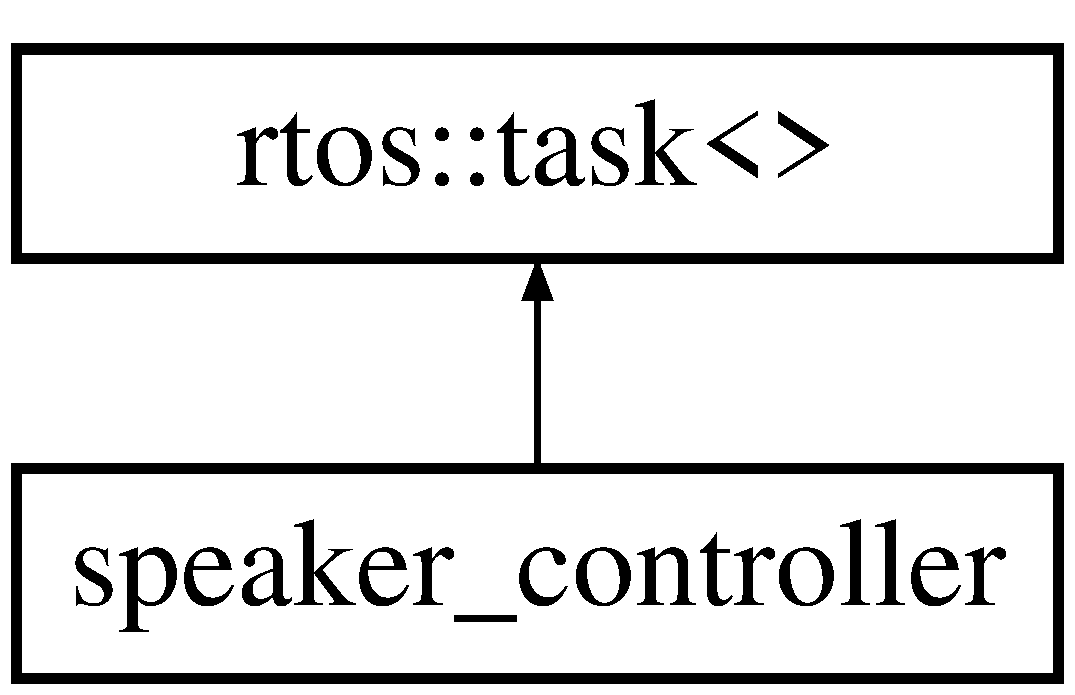
\includegraphics[height=2.000000cm]{classspeaker__controller}
\end{center}
\end{figure}
\subsection*{Public Member Functions}
\begin{DoxyCompactItemize}
\item 
\hyperlink{classspeaker__controller_aff5f11eb09fef5a599181d36a6b2a2a9}{speaker\+\_\+controller} (const char $\ast$task\+\_\+name, hwlib\+::pin\+\_\+out \&speaker\+\_\+pin, rtos\+::mutex \&sound\+\_\+mutex)
\begin{DoxyCompactList}\small\item\em Default constructor. \end{DoxyCompactList}\item 
void \hyperlink{classspeaker__controller_a13df562814c54591d83e4dd05e6930ca}{play\+\_\+sound} (const \hyperlink{structsound__lookup}{sound\+\_\+lookup} \&play)
\begin{DoxyCompactList}\small\item\em play sound \end{DoxyCompactList}\item 
void \hyperlink{classspeaker__controller_a7596b187aa529529886992fd6545bcab}{write} (const \hyperlink{structsound__lookup}{sound\+\_\+lookup} sound\+\_\+struct)
\begin{DoxyCompactList}\small\item\em write to sound pool \end{DoxyCompactList}\item 
void \hyperlink{classspeaker__controller_ac960be64207122d099dab24de3928d98}{enable\+\_\+flag} ()
\begin{DoxyCompactList}\small\item\em Set the play sound flag. \end{DoxyCompactList}\end{DoxyCompactItemize}
\subsection*{Public Attributes}
\begin{DoxyCompactItemize}
\item 
\hypertarget{classspeaker__controller_a35a3ec318694a96a19fa242fa061205b}{}\label{classspeaker__controller_a35a3ec318694a96a19fa242fa061205b} 
\hyperlink{structsound__lookup}{sound\+\_\+lookup} \hyperlink{classspeaker__controller_a35a3ec318694a96a19fa242fa061205b}{shoot} \{4000,40000, 3, 50\}
\begin{DoxyCompactList}\small\item\em shoot sound \hyperlink{structsound__lookup}{sound\+\_\+lookup} \end{DoxyCompactList}\item 
\hypertarget{classspeaker__controller_a188de8c71de428765cd73f0f66d6d44e}{}\label{classspeaker__controller_a188de8c71de428765cd73f0f66d6d44e} 
\hyperlink{structsound__lookup}{sound\+\_\+lookup} \hyperlink{classspeaker__controller_a188de8c71de428765cd73f0f66d6d44e}{hit} \{500,50000, 3,200\}
\begin{DoxyCompactList}\small\item\em hit sound \hyperlink{structsound__lookup}{sound\+\_\+lookup} \end{DoxyCompactList}\end{DoxyCompactItemize}


\subsection{Detailed Description}
Speaker controller class. 

This class is used for controlling the speaker and converting the \hyperlink{structsound__lookup}{sound\+\_\+lookup} struct received from the sound pool to useable variables. Speaker\+\_\+controller uses the concurrency mechanism pool with mutex for receiving which sound is needed to be played. It also uses a flag to know when a new sond is ready to be read from the pool and played. 

\subsection{Constructor \& Destructor Documentation}
\hypertarget{classspeaker__controller_aff5f11eb09fef5a599181d36a6b2a2a9}{}\label{classspeaker__controller_aff5f11eb09fef5a599181d36a6b2a2a9} 
\index{speaker\+\_\+controller@{speaker\+\_\+controller}!speaker\+\_\+controller@{speaker\+\_\+controller}}
\index{speaker\+\_\+controller@{speaker\+\_\+controller}!speaker\+\_\+controller@{speaker\+\_\+controller}}
\subsubsection{\texorpdfstring{speaker\+\_\+controller()}{speaker\_controller()}}
{\footnotesize\ttfamily speaker\+\_\+controller\+::speaker\+\_\+controller (\begin{DoxyParamCaption}\item[{const char $\ast$}]{task\+\_\+name,  }\item[{hwlib\+::pin\+\_\+out \&}]{speaker\+\_\+pin,  }\item[{rtos\+::mutex \&}]{sound\+\_\+mutex }\end{DoxyParamCaption})\hspace{0.3cm}{\ttfamily [inline]}}



Default constructor. 

This constructor receives a task name, speaker pin and sound mutex as parameters. It initializes these together with the flag and pool. 

\subsection{Member Function Documentation}
\hypertarget{classspeaker__controller_ac960be64207122d099dab24de3928d98}{}\label{classspeaker__controller_ac960be64207122d099dab24de3928d98} 
\index{speaker\+\_\+controller@{speaker\+\_\+controller}!enable\+\_\+flag@{enable\+\_\+flag}}
\index{enable\+\_\+flag@{enable\+\_\+flag}!speaker\+\_\+controller@{speaker\+\_\+controller}}
\subsubsection{\texorpdfstring{enable\+\_\+flag()}{enable\_flag()}}
{\footnotesize\ttfamily void speaker\+\_\+controller\+::enable\+\_\+flag (\begin{DoxyParamCaption}{ }\end{DoxyParamCaption})\hspace{0.3cm}{\ttfamily [inline]}}



Set the play sound flag. 

This function is used to make other objects able to set the play sound flag. It returns nothing and requires no parameters. \hypertarget{classspeaker__controller_a13df562814c54591d83e4dd05e6930ca}{}\label{classspeaker__controller_a13df562814c54591d83e4dd05e6930ca} 
\index{speaker\+\_\+controller@{speaker\+\_\+controller}!play\+\_\+sound@{play\+\_\+sound}}
\index{play\+\_\+sound@{play\+\_\+sound}!speaker\+\_\+controller@{speaker\+\_\+controller}}
\subsubsection{\texorpdfstring{play\+\_\+sound()}{play\_sound()}}
{\footnotesize\ttfamily void speaker\+\_\+controller\+::play\+\_\+sound (\begin{DoxyParamCaption}\item[{const \hyperlink{structsound__lookup}{sound\+\_\+lookup} \&}]{play }\end{DoxyParamCaption})\hspace{0.3cm}{\ttfamily [inline]}}



play sound 

This function plays the sound from a received sound lookup. It calls the play function from the sound device. The function returns nothing. \hypertarget{classspeaker__controller_a7596b187aa529529886992fd6545bcab}{}\label{classspeaker__controller_a7596b187aa529529886992fd6545bcab} 
\index{speaker\+\_\+controller@{speaker\+\_\+controller}!write@{write}}
\index{write@{write}!speaker\+\_\+controller@{speaker\+\_\+controller}}
\subsubsection{\texorpdfstring{write()}{write()}}
{\footnotesize\ttfamily void speaker\+\_\+controller\+::write (\begin{DoxyParamCaption}\item[{const \hyperlink{structsound__lookup}{sound\+\_\+lookup}}]{sound\+\_\+struct }\end{DoxyParamCaption})\hspace{0.3cm}{\ttfamily [inline]}}



write to sound pool 

This function is used to make sure other classes can write to the sound pool. It returns nothing and requires a sound lookup type as parameter. 

The documentation for this class was generated from the following file\+:\begin{DoxyCompactItemize}
\item 
\hyperlink{speaker__classes_8hpp}{speaker\+\_\+classes.\+hpp}\end{DoxyCompactItemize}

\chapter{File Documentation}
\hypertarget{application__logic__classes_8hpp}{}\section{application\+\_\+logic\+\_\+classes.\+hpp File Reference}
\label{application__logic__classes_8hpp}\index{application\+\_\+logic\+\_\+classes.\+hpp@{application\+\_\+logic\+\_\+classes.\+hpp}}
\subsection*{Classes}
\begin{DoxyCompactItemize}
\item 
class \hyperlink{classir__message__logic}{ir\+\_\+message\+\_\+logic}
\begin{DoxyCompactList}\small\item\em Ir message logic class. \end{DoxyCompactList}\end{DoxyCompactItemize}

\hypertarget{display__classes_8hpp}{}\section{display\+\_\+classes.\+hpp File Reference}
\label{display__classes_8hpp}\index{display\+\_\+classes.\+hpp@{display\+\_\+classes.\+hpp}}
{\ttfamily \#include \char`\"{}hwlib.\+hpp\char`\"{}}\newline
{\ttfamily \#include \char`\"{}rtos.\+hpp\char`\"{}}\newline
\subsection*{Classes}
\begin{DoxyCompactItemize}
\item 
struct \hyperlink{structlcd__passthrough}{lcd\+\_\+passthrough}
\begin{DoxyCompactList}\small\item\em Lcd line structure. \end{DoxyCompactList}\item 
class \hyperlink{classlcd__display}{lcd\+\_\+display}
\begin{DoxyCompactList}\small\item\em display class \end{DoxyCompactList}\item 
class \hyperlink{classlcd__display__controller}{lcd\+\_\+display\+\_\+controller}
\begin{DoxyCompactList}\small\item\em Display controller. \end{DoxyCompactList}\end{DoxyCompactItemize}

\hypertarget{entity__classes_8hpp}{}\section{entity\+\_\+classes.\+hpp File Reference}
\label{entity__classes_8hpp}\index{entity\+\_\+classes.\+hpp@{entity\+\_\+classes.\+hpp}}
{\ttfamily \#include \char`\"{}hwlib.\+hpp\char`\"{}}\newline
\subsection*{Classes}
\begin{DoxyCompactItemize}
\item 
class \hyperlink{classmy__player__information}{my\+\_\+player\+\_\+information}
\begin{DoxyCompactList}\small\item\em Save the player information. \end{DoxyCompactList}\item 
class \hyperlink{classgame__information__data}{game\+\_\+information\+\_\+data}
\begin{DoxyCompactList}\small\item\em Store game information. \end{DoxyCompactList}\item 
class \hyperlink{classhit}{hit}
\begin{DoxyCompactList}\small\item\em Store a hit. \end{DoxyCompactList}\end{DoxyCompactItemize}

\hypertarget{game__time__classes_8hpp}{}\section{game\+\_\+time\+\_\+classes.\+hpp File Reference}
\label{game__time__classes_8hpp}\index{game\+\_\+time\+\_\+classes.\+hpp@{game\+\_\+time\+\_\+classes.\+hpp}}
{\ttfamily \#include \char`\"{}hwlib.\+hpp\char`\"{}}\newline
{\ttfamily \#include \char`\"{}rtos.\+hpp\char`\"{}}\newline
{\ttfamily \#include \char`\"{}entity\+\_\+classes.\+hpp\char`\"{}}\newline
{\ttfamily \#include \char`\"{}display\+\_\+classes.\+hpp\char`\"{}}\newline
\subsection*{Classes}
\begin{DoxyCompactItemize}
\item 
class \hyperlink{classgame__time__controller}{game\+\_\+time\+\_\+controller}
\begin{DoxyCompactList}\small\item\em Game time controller. \end{DoxyCompactList}\end{DoxyCompactItemize}

\hypertarget{init__game_8hpp}{}\section{init\+\_\+game.\+hpp File Reference}
\label{init__game_8hpp}\index{init\+\_\+game.\+hpp@{init\+\_\+game.\+hpp}}
{\ttfamily \#include \char`\"{}rtos.\+hpp\char`\"{}}\newline
{\ttfamily \#include \char`\"{}hwlib.\+hpp\char`\"{}}\newline
{\ttfamily \#include \char`\"{}keypad\+\_\+class.\+hpp\char`\"{}}\newline
{\ttfamily \#include \char`\"{}display\+\_\+classes.\+hpp\char`\"{}}\newline
{\ttfamily \#include \char`\"{}application\+\_\+logic\+\_\+classes.\+hpp\char`\"{}}\newline
{\ttfamily \#include \char`\"{}send\+\_\+ir\+\_\+classes.\+hpp\char`\"{}}\newline
\subsection*{Classes}
\begin{DoxyCompactItemize}
\item 
class \hyperlink{classinit__game__controller}{init\+\_\+game\+\_\+controller}
\begin{DoxyCompactList}\small\item\em Inialize the game. \end{DoxyCompactList}\end{DoxyCompactItemize}

\hypertarget{ir_01sender_01with_01channel_2send__ir__classes_8hpp}{}\section{ir sender with channel/send\+\_\+ir\+\_\+classes.hpp File Reference}
\label{ir_01sender_01with_01channel_2send__ir__classes_8hpp}\index{ir sender with channel/send\+\_\+ir\+\_\+classes.\+hpp@{ir sender with channel/send\+\_\+ir\+\_\+classes.\+hpp}}
{\ttfamily \#include \char`\"{}hwlib.\+hpp\char`\"{}}\newline
{\ttfamily \#include \char`\"{}rtos.\+hpp\char`\"{}}\newline
\subsection*{Classes}
\begin{DoxyCompactItemize}
\item 
class \hyperlink{classir__sender}{ir\+\_\+sender}
\begin{DoxyCompactList}\small\item\em Ir sender class. \end{DoxyCompactList}\item 
class \hyperlink{classsend__controller}{send\+\_\+controller}
\begin{DoxyCompactList}\small\item\em Ir send controller. \end{DoxyCompactList}\end{DoxyCompactItemize}

\hypertarget{ir_01sender_01with_01flag_2send__ir__classes_8hpp}{}\section{ir sender with flag/send\+\_\+ir\+\_\+classes.hpp File Reference}
\label{ir_01sender_01with_01flag_2send__ir__classes_8hpp}\index{ir sender with flag/send\+\_\+ir\+\_\+classes.\+hpp@{ir sender with flag/send\+\_\+ir\+\_\+classes.\+hpp}}
{\ttfamily \#include \char`\"{}hwlib.\+hpp\char`\"{}}\newline
{\ttfamily \#include \char`\"{}entity\+\_\+classes.\+hpp\char`\"{}}\newline
{\ttfamily \#include \char`\"{}rtos.\+hpp\char`\"{}}\newline
\subsection*{Classes}
\begin{DoxyCompactItemize}
\item 
class \hyperlink{classir__sender}{ir\+\_\+sender}
\begin{DoxyCompactList}\small\item\em Ir sender class. \end{DoxyCompactList}\item 
class \hyperlink{classsend__controller}{send\+\_\+controller}
\begin{DoxyCompactList}\small\item\em Ir send controller. \end{DoxyCompactList}\end{DoxyCompactItemize}

\hypertarget{ir__receiver__classes_8hpp}{}\section{ir\+\_\+receiver\+\_\+classes.\+hpp File Reference}
\label{ir__receiver__classes_8hpp}\index{ir\+\_\+receiver\+\_\+classes.\+hpp@{ir\+\_\+receiver\+\_\+classes.\+hpp}}
{\ttfamily \#include \char`\"{}hwlib.\+hpp\char`\"{}}\newline
{\ttfamily \#include \char`\"{}run\+\_\+game.\+hpp\char`\"{}}\newline
\subsection*{Classes}
\begin{DoxyCompactItemize}
\item 
class \hyperlink{classir__receiver__controller}{ir\+\_\+receiver\+\_\+controller}
\begin{DoxyCompactList}\small\item\em \hyperlink{classir__receiver__controller}{ir\+\_\+receiver\+\_\+controller} \end{DoxyCompactList}\end{DoxyCompactItemize}

\hypertarget{keypad__class_8hpp}{}\section{keypad\+\_\+class.\+hpp File Reference}
\label{keypad__class_8hpp}\index{keypad\+\_\+class.\+hpp@{keypad\+\_\+class.\+hpp}}
{\ttfamily \#include \char`\"{}hwlib.\+hpp\char`\"{}}\newline
\subsection*{Classes}
\begin{DoxyCompactItemize}
\item 
class \hyperlink{class_keypad}{Keypad}
\begin{DoxyCompactList}\small\item\em \hyperlink{class_keypad}{Keypad} class. \end{DoxyCompactList}\end{DoxyCompactItemize}

\hypertarget{listenerpattern_8hpp}{}\section{listenerpattern.\+hpp File Reference}
\label{listenerpattern_8hpp}\index{listenerpattern.\+hpp@{listenerpattern.\+hpp}}
{\ttfamily \#include \char`\"{}hwlib.\+hpp\char`\"{}}\newline
{\ttfamily \#include \char`\"{}rtos.\+hpp\char`\"{}}\newline
\subsection*{Classes}
\begin{DoxyCompactItemize}
\item 
class \hyperlink{classbutton}{button}
\begin{DoxyCompactList}\small\item\em button \end{DoxyCompactList}\item 
class \hyperlink{classlistener}{listener}
\begin{DoxyCompactList}\small\item\em Listener. \end{DoxyCompactList}\item 
class \hyperlink{classbutton__controller}{button\+\_\+controller}
\begin{DoxyCompactList}\small\item\em \hyperlink{classbutton__controller}{button\+\_\+controller} \end{DoxyCompactList}\end{DoxyCompactItemize}

\hypertarget{register__game__parameters__class_8hpp}{}\section{register\+\_\+game\+\_\+parameters\+\_\+class.\+hpp File Reference}
\label{register__game__parameters__class_8hpp}\index{register\+\_\+game\+\_\+parameters\+\_\+class.\+hpp@{register\+\_\+game\+\_\+parameters\+\_\+class.\+hpp}}
{\ttfamily \#include \char`\"{}entity\+\_\+classes.\+hpp\char`\"{}}\newline
{\ttfamily \#include \char`\"{}application\+\_\+logic\+\_\+classes.\+hpp\char`\"{}}\newline
{\ttfamily \#include \char`\"{}keypad\+\_\+class.\+hpp\char`\"{}}\newline
\subsection*{Classes}
\begin{DoxyCompactItemize}
\item 
class \hyperlink{classregister__game__parameters__controller}{register\+\_\+game\+\_\+parameters\+\_\+controller}
\begin{DoxyCompactList}\small\item\em \hyperlink{classregister__game__parameters__controller}{register\+\_\+game\+\_\+parameters\+\_\+controller} \end{DoxyCompactList}\end{DoxyCompactItemize}

\hypertarget{rgb__led__classes_8hpp}{}\section{rgb\+\_\+led\+\_\+classes.\+hpp File Reference}
\label{rgb__led__classes_8hpp}\index{rgb\+\_\+led\+\_\+classes.\+hpp@{rgb\+\_\+led\+\_\+classes.\+hpp}}
{\ttfamily \#include \char`\"{}hwlib.\+hpp\char`\"{}}\newline
{\ttfamily \#include \char`\"{}rtos.\+hpp\char`\"{}}\newline
\subsection*{Classes}
\begin{DoxyCompactItemize}
\item 
struct \hyperlink{structled__color__behaviour}{led\+\_\+color\+\_\+behaviour}
\begin{DoxyCompactList}\small\item\em Provide led color information. \end{DoxyCompactList}\item 
class \hyperlink{classrgb__led}{rgb\+\_\+led}
\begin{DoxyCompactList}\small\item\em Rgb led. \end{DoxyCompactList}\item 
class \hyperlink{classled__controller}{led\+\_\+controller}
\begin{DoxyCompactList}\small\item\em Led controller class. \end{DoxyCompactList}\end{DoxyCompactItemize}

\hypertarget{run__game_8hpp}{}\section{run\+\_\+game.\+hpp File Reference}
\label{run__game_8hpp}\index{run\+\_\+game.\+hpp@{run\+\_\+game.\+hpp}}
{\ttfamily \#include \char`\"{}hwlib.\+hpp\char`\"{}}\newline
{\ttfamily \#include \char`\"{}rtos.\+hpp\char`\"{}}\newline
{\ttfamily \#include \char`\"{}display\+\_\+classes.\+hpp\char`\"{}}\newline
{\ttfamily \#include \char`\"{}register\+\_\+game\+\_\+parameters\+\_\+class.\+hpp\char`\"{}}\newline
{\ttfamily \#include \char`\"{}keypad\+\_\+class.\+hpp\char`\"{}}\newline
{\ttfamily \#include \char`\"{}game\+\_\+time\+\_\+classes.\+hpp\char`\"{}}\newline
{\ttfamily \#include \char`\"{}listenerpattern.\+hpp\char`\"{}}\newline
{\ttfamily \#include \char`\"{}speaker\+\_\+classes.\+hpp\char`\"{}}\newline
{\ttfamily \#include \char`\"{}rgb\+\_\+led\+\_\+classes.\+hpp\char`\"{}}\newline
{\ttfamily \#include \char`\"{}send\+\_\+ir\+\_\+classes.\+hpp\char`\"{}}\newline
\subsection*{Classes}
\begin{DoxyCompactItemize}
\item 
class \hyperlink{classrun__game__controller}{run\+\_\+game\+\_\+controller}
\begin{DoxyCompactList}\small\item\em run the game \end{DoxyCompactList}\end{DoxyCompactItemize}

\hypertarget{speaker__classes_8hpp}{}\section{speaker\+\_\+classes.\+hpp File Reference}
\label{speaker__classes_8hpp}\index{speaker\+\_\+classes.\+hpp@{speaker\+\_\+classes.\+hpp}}
{\ttfamily \#include \char`\"{}hwlib.\+hpp\char`\"{}}\newline
{\ttfamily \#include \char`\"{}rtos.\+hpp\char`\"{}}\newline
\subsection*{Classes}
\begin{DoxyCompactItemize}
\item 
struct \hyperlink{structsound__lookup}{sound\+\_\+lookup}
\begin{DoxyCompactList}\small\item\em Data structure for sound\+\_\+storage. \end{DoxyCompactList}\item 
class \hyperlink{classspeaker}{speaker}
\begin{DoxyCompactList}\small\item\em speaker class \end{DoxyCompactList}\item 
class \hyperlink{classspeaker__controller}{speaker\+\_\+controller}
\begin{DoxyCompactList}\small\item\em Speaker controller class. \end{DoxyCompactList}\end{DoxyCompactItemize}

%--- End generated contents ---

% Index
\backmatter
\newpage
\phantomsection
\clearemptydoublepage
\addcontentsline{toc}{chapter}{Index}
\printindex

\end{document}
